%\title{Modelo de Projeto de pesquisa}
%% abtex2-modelo-projeto-pesquisa.tex, v-1.9 laurocesar
%% Copyright 2012-2013 by abnTeX2 group at http://abntex2.googlecode.com/ 
%%
%% This work may be distributed and/or modified under the
%% conditions of the LaTeX Project Public License, either version 1.3
%% of this license or (at your option) any later version.
%% The latest version of this license is in
%%   http://www.latex-project.org/lppl.txt
%% and version 1.3 or later is part of all distributions of LaTeX
%% version 2005/12/01 or later.
%%
%% This work has the LPPL maintenance status `maintained'.
%% 
%% The Current Maintainer of this work is the abnTeX2 team, led
%% by Lauro César Araujo. Further information are available on 
%% http://abntex2.googlecode.com/
%%
%% This work consists of the files abntex2-modelo-projeto-pesquisa.tex
%% and abntex2-modelo-references.bib
%%

% ------------------------------------------------------------------------
% ------------------------------------------------------------------------
% abnTeX2: Modelo de Projeto de pesquisa em conformidade com 
% ABNT NBR 15287:2011 Informação e documentação - Projeto de pesquisa -
% Apresentação 
% ------------------------------------------------------------------------ 
% ------------------------------------------------------------------------

\documentclass[
	% -- opções da classe memoir --
	12pt,				% tamanho da fonte
	openright,			% capítulos começam em pág ímpar (insere página vazia caso preciso)
	oneside,			% para impressão em verso e anverso. Oposto a oneside
	a4paper,			% tamanho do papel. 
	% -- opções da classe abntex2 --
	%chapter=TITLE,		% títulos de capítulos convertidos em letras maiúsculas
	%section=TITLE,		% títulos de seções convertidos em letras maiúsculas
	%subsection=TITLE,	% títulos de subseções convertidos em letras maiúsculas
	%subsubsection=TITLE,% títulos de subsubseções convertidos em letras maiúsculas
	% -- opções do pacote babel --
	english,			% idioma adicional para hifenização
	french,				% idioma adicional para hifenização
	spanish,			% idioma adicional para hifenização
	brazil,				% o último idioma é o principal do documento
	]{abntex2}

% ---
% PACOTES
% ---

% ---
% Pacotes fundamentais 
% ---
\usepackage{lmodern}			% Usa a fonte Latin Modern
\usepackage[T1]{fontenc}		% Selecao de codigos de fonte.
\usepackage[utf8]{inputenc}		% Codificacao do documento (conversão automática dos acentos)
\usepackage{indentfirst}		% Indenta o primeiro parágrafo de cada seção.
\usepackage{color}				% Controle das cores
\usepackage{graphicx}			% Inclusão de gráficos
\usepackage{microtype} 			% para melhorias de justificação
\usepackage{verbatim}           %comentar trechos grandes
\usepackage{amsmath}
% \usepackage{xcolor} % Já é carregado na linha 164
\usepackage{tabularx}
%\usepackage{subfigure}
\usepackage{subcaption}
%adicionais
\usepackage{cleveref} %ref. cruzada
\usepackage{listings} %importar códigos


% ---[]
%\usepackage[opções]{subfigure}	
%\graphicspath{{Imagens/}}

\usepackage{placeins}
\usepackage{float}

% ---
% Pacotes adicionais, usados apenas no âmbito do Modelo Canônico do abnteX2
% ---
\usepackage{lipsum}				% para geração de dummy text
% ---

% ---
% Pacotes de citações
% ---
%\usepackage[brazilian,hyperpageref]{backref}	 % Paginas com as citações na bibl
%\usepackage[alf]{abntex2cite}	% Citações padrão ABNT
\usepackage[backend=biber, style=abnt]{biblatex}
\addbibresource{ref.bib}

\usepackage{csquotes} % Gerencia aspas
% --- 
% CONFIGURAÇÕES DE PACOTES
% --- 


%%%%%%%%%%%%%%%%%%%%%%%%%%%%%%%%%%%%%%%%%%%%%%%%%%%%%%%%%%%%%%

\definecolor{mygreen}{RGB}{28,172,0} % color values Red, Green, Blue
\definecolor{mylilas}{RGB}{170,55,241}
\definecolor{codegreen}{rgb}{0,0.6,0}
\definecolor{codegray}{rgb}{0.5,0.5,0.5}
\definecolor{codepurple}{rgb}{0.58,0,0.82}
\definecolor{backcolour}{rgb}{0.95,0.95,0.92}
\definecolor{azul}{rgb}{0, 0, 255}
\definecolor{Cyan}{rgb}{0, 100,0}
\definecolor{fundo}{rgb}{29, 41, 81}

\lstdefinestyle{mystyle}{
  backgroundcolor=\color{backcolour},   commentstyle=\color{codegreen},
  keywordstyle=\color{magenta},
  numberstyle=\tiny\color{codegray},
  stringstyle=\color{codepurple},
  basicstyle=\footnotesize,
  breakatwhitespace=false,         
  breaklines=true,                 
  captionpos=b,                    
  keepspaces=true,                 
  numbers=left,                    
  numbersep=5pt,                  
  showspaces=false,                
  showstringspaces=false,
  showtabs=false,                  
  tabsize=2
}

\lstset{language=Matlab,%
    %basicstyle=\color{red},
    breaklines=true,%
    morekeywords={matlab2tikz},
    keywordstyle=\color{blue},%
    morekeywords=[2]{1}, keywordstyle=[2]{\color{black}},
    identifierstyle=\color{black},%
    stringstyle=\color{mylilas},
    commentstyle=\color{mygreen},%
    showstringspaces=false,%without this there will be a symbol in the places where there is a space
    numbers=left,%
    numberstyle={\tiny \color{black}},% size of the numbers
    numbersep=9pt, % this defines how far the numbers are from the text
    emph=[1]{for,end,break},emphstyle=[1]\color{red}, %some words to emphasise
    %emph=[2]{word1,word2}, emphstyle=[2]{style},    
}

\lstset{style=mystyle,
literate=
{á}{{\'a}}1
{à}{{\`a}}1
{ã}{{\~a}}1
{é}{{\'e}}1
{ê}{{\^e}}1
{í}{{\'i}}1
{ó}{{\'o}}1
{õ}{{\~o}}1
{ú}{{\'u}}1
{ü}{{\"u}}1
{ç}{{\c{c}}}1
}

% Please add the following required packages to your document preamble:
\usepackage[table,xcdraw]{xcolor}

% If you use beamer only pass "xcolor=table" option, 
% \documentclass[xcolor=table]{beamer} % --- DUAS CLASSES DE DOCUMENTO LEVANTAM ERROS NO COMPILADOR --- %
%%%%%%%%%%%%%%%%%%%%%%%%%%%%%%%%%%%%%%%%%%%%%%%%%%%%%%

% ---
% Informações de dados para CAPA e FOLHA DE ROSTO
% ---
\titulo{Projeto de Máquinas: Torno CNC}
\autor{Breno Martins Braga --- NUSP 12556288 \\
		Constanza Maria Reis da Silva Mariano --- NUSP 11257884\\
        Douglas Oliveira de Carvalho --- NUSP 14637740\\
        Fernanda Quelho Kaiser Saliba Andrade --- NUSP 11258162\\
        Gabriel Morth Cursino NUSP --- 12553250 \\
        Gabriel Silva de Carvalho -- NUSP 12730737 \\
        Hassan Mohamad Vilela --- NUSP 11257904 \\
        Jhonatan Ribeiro dos Santos --- NUSP 12554477 \\
        Mario Lourenço Fernandes --- NUSP 11807730 \\
        Soitiro Oura --- NUSP 12554265 \\
        Vinícios de Andrade Cardozo --- NUSP 12554290}
\local{PMR3411 - Projeto de Máquinas\\
Escola Politécnica da Universidade de São Paulo}
\data{17 de novembro, 2024} % Data da última modificação, atualizar antes da entrega final 

\instituicao{%
  Universidade de São Paulo
  \par
  Escola Politécnica}
\tipotrabalho{Relatório}
% O preambulo deve conter o tipo do trabalho, o objetivo, 
% o nome da instituição e a área de concentração 
%%\preambulo{Minicurso de aplicação do modelo \abnTeX \;
%%com as normas ABNT apresentado à comunidade de usuários \LaTeX.}
% ---

% ---
% Configurações de aparência do PDF final

% alterando o aspecto da cor azul
\definecolor{blue}{RGB}{41,5,195}

% informações do PDF
\makeatletter
\hypersetup{
     	%pagebackref=true,
		pdftitle={\@title}, 
		pdfauthor={\@author},
    	pdfsubject={\imprimirpreambulo},
	    pdfcreator={LaTeX with abnTeX2},
		pdfkeywords={abnt}{latex}{abntex}{abntex2}{projeto de pesquisa}, 
		colorlinks=true,       		% false: boxed links; true: colored links
    	linkcolor=black,          	% color of internal links
    	citecolor=black,        		% color of links to bibliography
    	filecolor=magenta,      		% color of file links
		urlcolor=black,
		bookmarksdepth=4
}
\makeatother
% --- 

% --- 
% Espaçamentos entre linhas e parágrafos 
% --- 

% O tamanho do parágrafo é dado por:
\setlength{\parindent}{1.3cm}

% Controle do espaçamento entre um parágrafo e outro:
\setlength{\parskip}{0.2cm}  % tente também \onelineskip

% ---
% compila o indice
% ---
\makeindex
% ---

% ----
% Início do documento
% ----
\begin{document}


% Retira espaço extra obsoleto entre as frases.
\frenchspacing 

% ----------------------------------------------------------
% ELEMENTOS PRÉ-TEXTUAIS
% ----------------------------------------------------------
% \pretextual

% ---
% Capa
% ---
\imprimircapa
% ---

% ---
% Folha de rosto
% ---
%\imprimirfolhaderosto
% ---

% ---
% NOTA DA ABNT NBR 15287:2011, p. 4:
%  ``Se exigido pela entidade, apresentar os dados curriculares do autor em
%     folha ou página distinta após a folha de rosto.''
% ---

% ---
% inserir lista de ilustrações
% ---
\pdfbookmark[0]{\listfigurename}{lof}
\listoffigures*
\cleardoublepage
% ---

% ---
% inserir lista de tabelas
% ---
\pdfbookmark[0]{\listtablename}{lot}
\listoftables*
\cleardoublepage
% ---

% ---
% inserir o sumario
% ---
\pdfbookmark[0]{\contentsname}{toc}
\tableofcontents*
\cleardoublepage
% ---


% ----------------------------------------------------------
% ELEMENTOS TEXTUAIS
% ----------------------------------------------------------
\textual

% ----------------------------------------------------------
% Introdução
% ----------------------------------------------------------


\chapter{Introdução}

\setcounter{page}{1}


\section{Subgrupos}

Para obter uma otimização na organização do projeto, e garantir uma divisão justa e igual para todos os membros, o grupo se dividiu em subgrupos, cada um responsável por uma parte importante do projeto. É importante ressaltar que os membros da equipe são responsáveis por ajudar em todas as partes do trabalho, não somente o subgrupo em que está inserido, de forma que seja possível uma boa comunicação entre os times. A divisão dos subgrupos escolhida foi a seguinte:

\begin{itemize}
    \item \textbf{Gerência:} a gerente do grupo é responsável por garantir uma boa organização do trabalho como um todo, além de verificar se todos os membros do grupo estão participando do projeto.
    \item \textbf{Mecânica:} este subgrupo tem como função garantir o bom funcionamento da parte estrutural da máquina: desde o esboço inicial, passando pela escolha de materiais, até a montagem do protótipo.
    \item \textbf{Eletrônica:} esta equipe cuida de todos os componentes elétricos do torno, suas conexões e seu bom funcionamento.
    \item \textbf{Programação:} Este time deve realizar a parte da lógica de funcionamento e do código Linux CNC da máquina.
\end{itemize}

É notável que todos os subgrupos devem se comunicar entre si para o bom funcionamento do projeto, e é claro, trabalhar em conjunto para que a máquina funcione da maneira desejada.


\newpage
\chapter{Especificações de máquina}

Neste capítulo, são apresentados os materiais escolhidos e as especificações da máquina, como por exemplo o volume de trabalho, a precisão e a velocidade de usinagem, parâmetros essenciais para a compreensão do funcionamento de um torno.

\section{Materiais}

Dentre os materiais disponíveis, esse grupo selecionou os seguintes: 
\begin{itemize}
    \item Inversor CFM 500
    \item Correia sincronizadora Optibelt ZR 345L
    \item Polia 26 L 075 
    \item Polia 48 L 075
    \item Mesa deslizante 3 (430 mm) e 4 (280 mm)
    \item 2x Motor KTC HT-23-400
    \item 2x Acoplamento fole (tipo 3)
\end{itemize}
%%%%%%%%%%%%%%%%%%%%%%%%%%%%%%%%%%%%%%%%%%%%%%%%%%%%%%%%%%%%%%%

\section{Eixo árvore}
O eixo árvore especificado para a máquina é composto por uma placa de três castanhas para fixação da peça, perfil tubular de aço com seção quadrada de 100 mm de lado e 3,18 mm de parede, rolamentos radiais de esferas, polia para correia sincronizadora e encoder óptico.

Seguem as imagens que especificam o funcionamento do encoder óptico e também o rolamento de esferas:

\begin{figure}[h!]
    \centering
    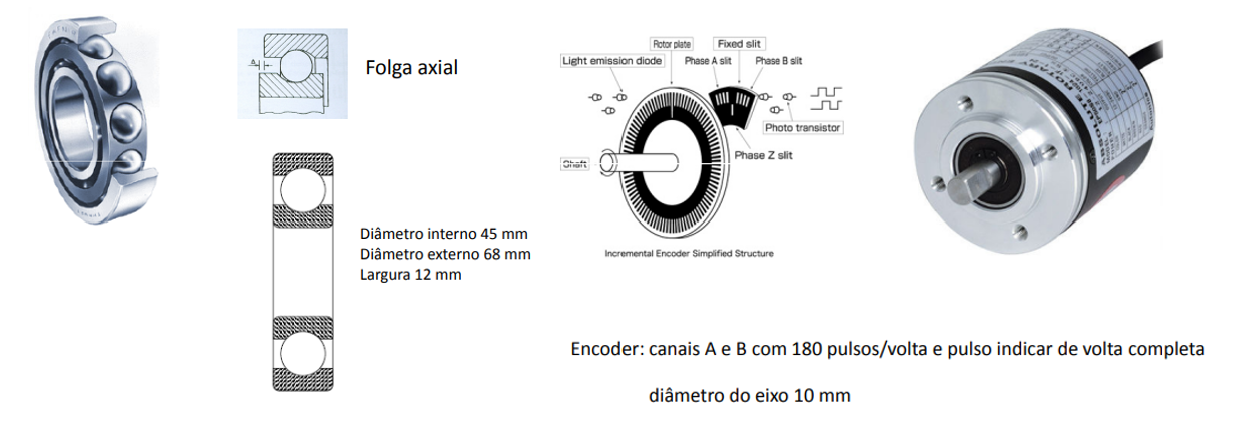
\includegraphics[width=\linewidth]{images/rolamentos.png}
    \label{fig:enter-label}
\end{figure}

\subsection{Potência}

De acordo com as especificações iniciais do motor CA que transmitirá movimento à máquina por meio da transmissão por correia, a sua potência fornecida é de 0,5 HP, dada uma tensão de 220V e uma rotação de 1720rpm.

As potências fornecidas pelo motor de passo, no entanto, variam de modelo para modelo. Considerando o motor KTC-HT23-401, temos diferentes valores a depender da operação (torque transmitido e respectiva velocidade angular). 

O motor KTC-HT23-400 possui uma curva de torque dada o valor do par revoluções por segundo e torque que transmite a maior potência para o sistema é um torque de 0,67Nm a uma rotação de 15 revoluções por segundo, que gera uma potência de 0,08468 HP.

\begin{figure}[h!]
    \centering
    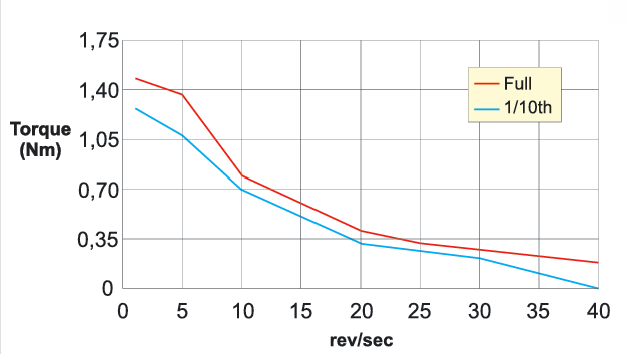
\includegraphics[width=0.8\linewidth]{images/torque.png}
    \caption{Curva de torque do motor de passo KTC-HT23-400 \cite{kalatec2020catalogo}.}
    \label{fig:enter-label}
\end{figure}

\subsection{Rotação}

Levando em consideração a tabela e sabendo que o inversor a ser utilizado armazena até 8 velocidades, podemos escolhê-las de acordo com a ferramenta, que será de aço rápido, e o material usinado, que será de material mole (para as presentes especificações utiliza-se o Nylon). Deve-se levar também em conta que a placa de castanhas possui limitação de rotação de 900 RPM. 

Considerando um peça de nylon de diâmetro máximo 100mm a rotação do eixo necessária, de acordo com a equação 21, na seção 13.1, para as operações de usinagem é 955 RPM. Esse valor aumentará de forma inversamente proporcional ao diâmetro a peça. 

As demais 8 rotações serão ainda escolhidas para cada processo (acabamento, desbaste e rosqueamento) e diâmetro disponível da peça. Em seguida, elas serão programadas no inversor para a usinagem das peças.  

%%%%%%%%%%%%%%%%%%%%%%%%%%%%%%%%%%%%%%%%%%%%%%%%%%%%%%%%%%%%%%%
\section{Especificações Elétricas}

Para as especificações elétricas foram analisados dados elétricos dos 2 tipos de motores utilizados: KTC - HT -23 - 400 e Motor CA 0,5 HP. 


\begin{table}
    \centering
    \begin{tabular}{|c|c|c|l|l|l|} \hline 
         &  Pot  [KW]& Tensão [V] & \multicolumn{3}{|c|}{Corrente [A]}\\ \hline 
         KTC-HT-23-400&  0,063&  31,5& 2,80& 2,00&1,40
\\ \hline 
         Motor CA 0.5 HP&  0,373&  220& -& 1,69&-
\\ \hline
    \end{tabular}
    \label{tab:my_label}
\end{table}

\subsection{Tensão e Corrente}
A máquina será alimentada com tensão e corrente adequadas para suportar os motores e outros componentes eletrônicos, garantindo a eficiência energética e a segurança operacional.

\subsection{Controlador}
O controlador escolhido para a máquina é o Linux CNC, que permitirá um controle preciso das operações. Será configurado para suportar a interface com os motores de passo e demais componentes eletrônicos.

As principais atividades que o dispositivo desempenhará serão:
\begin{itemize}
    \item Comunicação por portas paralelas
    \item Controle automático por código G
    \item Controle automático dos motores de passo sem feedback
    \item Controle automático da velocidade do eixo árvore com feedback de um encoder
    \item Controle manual utilizando um joystick
\end{itemize}

\subsection{Resolução}
Os motores de passo selecionados realizam 200 passos por volta, ou seja 1.8$^{\circ}$ por passo; Com o driver de micropasso temos 10x o número de passos por volta, logo 0.18$^{\circ}$ por passo.

Para ambas as nossas mesas deslizantes temos que seus fusos tem passo igual a 5mm ou uma vota completa, move a mesa 5mm.

\begin{equation}
   Resolução = \frac{\text{Passo}}{\text{Resolução do conjunto}} = \frac{5 mm/volta}{2000 steps/volta} = 2.5 \mu m /volta
\end{equation}

Portanto, a resolução máxima de movimentação de ambas as mesas deslizantes é de $2,5 \mu m$. Ou seja, esse valor corresponde ao menor incremento que o controle é capaz de executar.  

\subsection{Avanço rápido}

O avanço foi dimensionado para permitir deslocamentos ágeis entre os ciclos de usinagem, sem comprometer a precisão.

\subsection{Driver e Motor de Passo}
Será utilizado um driver de motor de passo do tipo micro passo com 2000 posições por volta, o que resulta em uma resolução angular de 0.18$^{\circ}$ por passo.
%%%%%%%%%%%%%%%%%%%%%%%%%%%%%%%%%%%%%%%%%%%%%%%%%%%%%%%%%%%%%%%
\section{Precisão e Acurácia}

Para o projeto da máquina busca-se uma precisão de usinagem de décimo de milímetro. Ambos fatores dependerão da construção da máquina como um todo. 

%%%%%%%%%%%%%%%%%%%%%%%%%%%%%%%%%%%%%%%%%%%%%%%%%%%%%%%%%%%%%%%
\section{Dimensões e Peso da Máquina}

Os materiais possuem os pesos listados abaixo, sendo que as diferentes soluções podem utilizar diferentes elementos, variando o seu peso total. Caso todos os componetentes sejam usados, o peso total assume $25.25$ kg. 

\begin{itemize}
    \item Mesas Deslizantes: 5 Kg (extraído do Catalogo do produto)
    \item Motores de passo: 2 Kg (extraído do Manual)
    \item Encoder: 0,4 Kg (extraído do datasheet)
    \item Motor CA: 10 Kg (Retirado do Catalogo do produto)
    \item Inversor: 1 Kg (extraído do Manual do usuário)
    \item Polias: 2,9 Kg (extraído do Manual)
    \item Rolamento eixo árvore: 0,15 Kg (Catálogo)
    \item Acoplamento Tipo Fole:  $ \lt $  0,1 Kg
    \item Correias Sincronizadoras: $ \lt $ 0,5 Kg (material é feito de borracha)
    \item Placa de três castanhas: 3,2 Kg (Especificação da peça)
\end{itemize}

%%%%%%%%%%%%%%%%%%%%%%%%%%%%%%%%%%%%%%%%%%%%%%%%%%%%%%%%%%%%%%%%
\newpage
\section{Cursos e velocidades dos eixos}

Os cursos e as velocidades dos eixos da máquina foram projetados para garantir uma usinagem eficiente e precisa. Abaixo estão as especificações para cada eixo:

\subsection{Cursos dos Eixos}
O torno utilizará blocos deslizantes nos eixos Z e X com comprimentos 540mm e 430mm, respectivamente. Os cursos máximos de fim de curso é descrito na seção abaixo. 

Nos dois eixos o movimento será realizado por um fuso de esferas recirculantes (com passo de 5mm) acoplado a um motor de passo. 

\section{Volume de trabalho}
Corresponde a área máxima que a peça poderia dentro de uma área útil de trabalho.

\begin{figure}[h!]
    \centering
    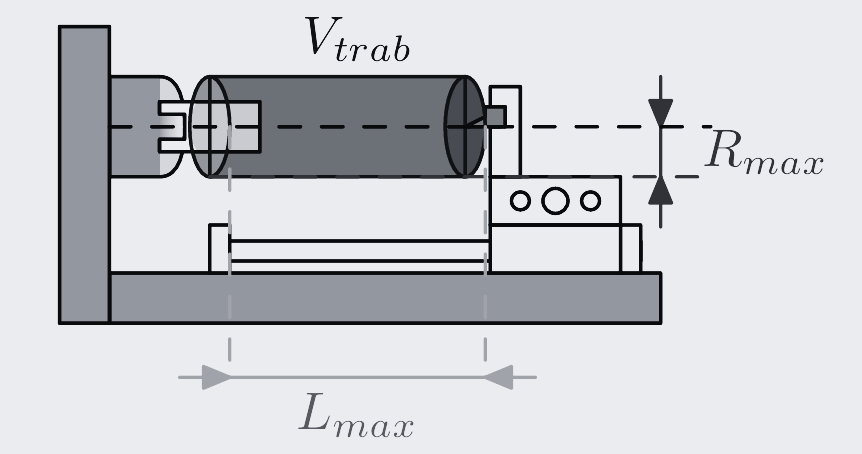
\includegraphics[width=0.8\linewidth]{images/vtrab.png}
    \caption{Representação gráfica do cálculo de volume de trabalho. Fonte: Autor.}
    \label{fig:vtrab}
\end{figure}

$$V_{trab} =(\pi R^2 Max) \cdot L_{Max}$$

$$R_{Max} = 50[mm]$$

$$L_{Max} = \text{Distância entre furos - Comprimento da mesa - Tamanho de um apoio}$$

$$L_{Max} =430[mm] - 130[mm] - 20[mm]$$

$$L_{Max} = 280[mm]$$

$$V_{trab} =(\pi \cdot 502) \cdot 280 = 2.199.114,86[mm^3]$$

$$V_{trab} = 0,0022[m^3]$$

\subsection{Velocidades dos Eixos}

O motor de passo KTC-HT23-400 apresenta uma relação inversa entre torque e velocidade, ou seja, à medida que o torque aumenta, a velocidade de rotação diminui. Quando se exige mais torque, a inércia do sistema também precisa ser minimizada para evitar perdas de eficiência e garantir que o motor funcione de maneira adequada.

A seguir, apresenta-se uma tabela que correlaciona os valores de velocidade e torque em função da massa móvel. Essa tabela fornece uma visão clara de como diferentes massas e torques impactam a velocidade e, consequentemente, a aceleração do sistema. A partir desses dados, será possível determinar os coeficientes de aceleração ideais para cada situação, garantindo que o motor funcione de forma eficiente e segura.

Para a obtenção da tabela, usaram as seguintes fórmulas: 
\begin{equation}
    J_{massa} = (m_{mesa} + m_{peca}) \cdot (\frac{p}{2\pi})^2
\end{equation}, para o cálculo do momento de inércia da carga. 

\begin{equation}
    J_{fuso} = \frac{1}{2} \cdot m_{fuso} \cdot (\frac{d_{fuso}}{2})^2
\end{equation}, para o cálculo do momento de inércia do fuso. 

Baseado na curva de torque da Seção 4.1, percebe-se que a velocidade do motor estará bem próxima da máxima, ou seja, 40[rev/s] e como o passo é 5[mm] temos que a velocidade dos eixos x e z em m/s é 0.2[m/s]. A velocidade média é de 0.1[m/s].  

Para estimar o momento de inércia do motor a partir da curva de torque versus velocidade, usou-se a relação entre o torque e a aceleração angular, dada pela equação:

\begin{equation}
    T = J \cdot \dot{\omega}
\end{equation}

Onde:
\begin{itemize}
    \item \( T \) é o torque (Nm),
    \item \( J \) é o momento de inércia (em kg $\cdot m^2$),
    \item \( \dot{\omega} \) é a aceleração angular (em $\frac{rad}{s^2}$).
\end{itemize}

A partir da curva, podemos identificar que o torque máximo \( T \) no modo Full Step é aproximadamente \( 1.4 \, \text{Nm} \), e a velocidade máxima do motor é \( 40 \, \text{rev/s} \). Para converter a velocidade em \( \text{rad/s} \), usamos a seguinte fórmula:

\begin{equation}
    \omega = 2\pi \cdot 40 \ = 251.2 \, \text{rad/s}
\end{equation}

Supondo que o motor acelere de \( 0 \, \text{rad/s} \) até \( 251.2 \, \text{rad/s} \) em \( 2 \, \text{segundos} \). A aceleração angular é então dada por:

\begin{equation}
    \dot{\omega} = \frac{\Delta \omega}{\Delta t} = \frac{251.2}{2} \, \text{rad/s²} = 125.6 \, \text{rad/s²}
\end{equation}

Substituindo os valores de \( T \) e \( \dot{\omega} \) na equação para o torque:

\begin{equation}
    1.4 = J \cdot 125.6
\end{equation}

Agora, resolvemos para \( J \):

\begin{equation}
    J = \frac{1.4}{125.6} = 0.01114 \, \text{kg} \cdot \text{m}^2
\end{equation}

Assim, o momento de inércia estimado do motor é aproximadamente:

\begin{equation}
    J_{motor} \approx 0.011 \, \text{kg} \cdot \text{m}^2
\end{equation}

A inércia acelerada será, portanto, 

\begin{equation}
    J_{carga} = J_{massa} + J_{fuso} + J_{motor} + J_{acoplamento} 
\end{equation}

Por fim, o torque de acionamento será obtido através da expressão:

\begin{equation}
    T_{acionamento} = J_{carga} \cdot \dot \omega + T_{atrito}
\end{equation}

Para o cálculo do torque de atrito, consideram-se aqueles gerados pelas guias lineareas, os mais de rolamento e os fusos. 

\begin{align}
    T_{guias} = \frac{p}{2\pi} \cdot \mu_{guias} \cdot [g(m_{mesa}+m_{peca})+F_{NormalCorte}] \\
    T_{mancal} = \mu \cdot \frac{d_{internoMancal}}{2} \cdot (F_{corte}+F_{préCarga}) \\
    T_{fuso} = \frac{p}{2\pi}\cdot F_{corte} \\
\end{align}

O torque de atrito final, portante, será dado pela expressão: 
\begin{equation}
    T = T_{guia} + T_{mancais} + T_{fuso}
\end{equation}

Por fim, chegou-se nos resultados da tabela abaixo. 

\begin{table}[h!] 
    \centering 
    \begin{tabular}{|c|c|c|} \hline 
        \textbf{Massa móvel [kg]} & \textbf{Torque [N.m]} & \textbf{Velocidade angular [rad/s]} \\ \hline 
        5 & 0,65 & 180 \\ \hline 
        8 & 0,80 & 160 \\ \hline 
        10 & 1,05 & 130 \\ \hline 
        12 & 1,25 & 110 \\ \hline 
    \end{tabular} 
    \caption{Correlação entre Massa Móvel, Torque e Velocidade Angular}  
\end{table}

A partir da análise da tabela, percebe-se que uma velocidade mais baixa requer um torque mais elevado, pois a resistência mecânica ou a carga aplicada ao motor aumenta. Nesses casos, o motor precisa aplicar mais força (torque) para continuar girando, o que pode comprometer a velocidade máxima atingível. Portanto, ao projetar a dinâmica do sistema, é essencial encontrar um equilíbrio entre torque, inércia e velocidade, ajustando os parâmetros de aceleração para que o motor atinja o torque necessário sem prejudicar a eficiência do sistema.

%%%%%%%%%%%%%%%%%%%%%%%%%%%%%%%%%%%%%%%%%%%%%%%%%%%%%%%%%%%%%%%%
\newpage
\section{Frequência Crítica do Laço Estrutural}

A frequência máxima de operação é de 30 Hz, limitada pelos motores utilizados, garantindo que a máquina opere abaixo de sua frequência natural para evitar ressonâncias.

%%%%%%%%%%%%%%%%%%%%%%%%%%%%%%%%%%%%%%%%%%%%%%%%%%%%%%5
\section{Tipo de sincronização entre os eixos}

Os movimentos dos eixos de uma máquina (como um torno ou fresadora) são coordenados para garantir que eles trabalhem em harmonia durante a operação. A sincronização é essencial para garantir a precisão nos processos de usinagem, já que o movimento de um eixo pode afetar diretamente o movimento do outro, especialmente em operações que requerem alta precisão.

A sincronização entre os eixos será feita por meio de uma \textbf{correia sincronizadora}. Ela é responsável por transmitir o movimento de forma simultânea entre os eixos, mantendo uma relação de velocidade constante. 

No presente projeto, a correia Optibelt ZR 345L cumpre essa função ao garantir que o movimento de um eixo seja replicado em outro de forma precisa, sem escorregamento, já que as correias sincronizadoras possuem dentes que se encaixam perfeitamente nas polias, evitando desvios.

Dentre as vantagens de utilizar esse tipo de sincronização entre eixos, é que esse é silencioso, requer pouca manutenção e oferece bom desempenho em termos de durabilidade e precisão.

%%%%%%%%%%%%%%%%%%%%%%%%%%%%%%%%%%%%%%%%%%%%%%%%%%%%%%%%%%%%%%%%

\section{Parâmetros de usinagem}

\subsection{Velocidade de corte}

A velocidade de corte refere-se à distância que a ferramenta percorre ao cortar o material em um determinado período de tempo. Esse parâmetro é crucial na operação de usinagem em um torno, pois permite calcular a rotação, em RPM, da placa de castanha, responsável por gerar a velocidade de corte no material. A velocidade de corte é determinada pela seguinte fórmula:

\begin{equation}
n=\frac{V_{C} \cdot 1000}{\pi d}    
\end{equation}

Onde: \\
- n  = rotação da máquina, em RPM; \\
- $\V_{C}$ = velocidade de corte, em m/min; \\
- d = diâmetro da peça, em mm. \\

Embora existam fórmulas para calcular a velocidade de corte, ela é frequentemente obtida em tabelas que já relacionam a operação, o material a ser usinado e o tipo de ferramenta de corte utilizada.

\begin{figure}[h!]
    \centering
    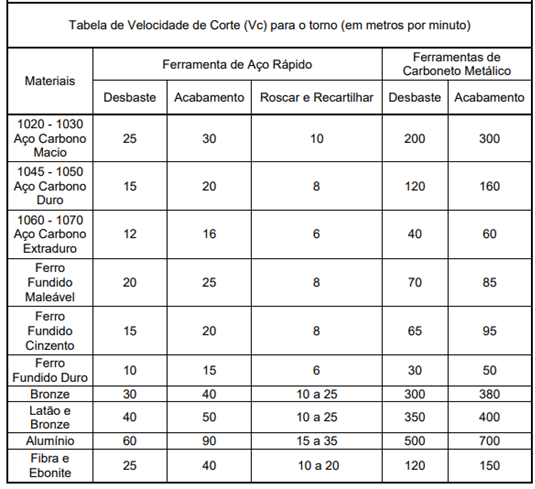
\includegraphics[width=0.7\linewidth]{images/vc_torno.png}
    \caption{Tabela de velocidade de corte para o torno (m/min).}
    \label{fig:enter-label}
\end{figure}

O Nylon 6.0 não está especificado na tabela acima, portanto, realizou-se uma pesquisa em sites de fabricantes de Nylon 6.0. De acordo com essas fontes, a velocidade de corte recomendada para o material varia entre 50 e 500 m/min, dependendo da operação realizada. Para o desbaste, utilizaremos uma velocidade de corte de 300 m/min. Com base nesse valor, é possível calcular a rotação necessária para usinar três tarugos de diferentes diâmetros: 25 mm, 50 mm e 100 mm.

Abaixo estão os cálculos da rotação necessária para manter a velocidade de corte de 300 m/min em cada um dos casos \cite{nylon6datasheet}:

Para 25mm de diâmetro:

\begin{align}
n=\frac{V_{C} \cdot 1000}{\pi d} = \frac{300 \cdot 1000}{\pi \cdot 25} = 3822 \text{rpm}
\end{align}

Para 50mm de diâmetro:

\begin{align}
n=\frac{V_{C} \cdot 1000}{\pi d} = \frac{300 \cdot 1000}{\pi \cdot 50} = 1911 \text{rpm}  
\end{align}

Para 100mm de diâmetro:

\begin{align}
n=\frac{V_{C} \cdot 1000}{\pi d} = \frac{300 \cdot 1000}{\pi \cdot 100} = 955 \text{rpm}
\end{align}

Esses valores são fundamentais, pois a utilização de velocidades de corte inadequadas na usinagem pode gerar diversos problemas. Quando a velocidade de corte está acima da recomendada, pode ocorrer o superaquecimento tanto da peça quanto da ferramenta, além da perda do fio de corte da ferramenta. Por outro lado, uma velocidade de corte abaixo do recomendado pode causar o travamento da ferramenta, muitas vezes resultando em sua quebra.

\subsection{Avanço de corte}

O avanço de corte representa a relação entre a velocidade de deslocamento da ferramenta e a velocidade da peça por rotação do eixo da máquina (mm/rotação). Ele depende diretamente da escolha da velocidade de corte, e, após essa definição, é necessário selecionar o avanço de corte adequado.
Assim como a velocidade de corte, o avanço de corte é fornecido por meio de tabelas disponibilizadas pelos fabricantes de ferramentas. Essas tabelas relacionam o material a ser usinado, o material da ferramenta e o tipo de operação a ser realizada. Abaixo está um exemplo de tabela de avanços de corte:

\begin{figure}[h!]
    \centering
    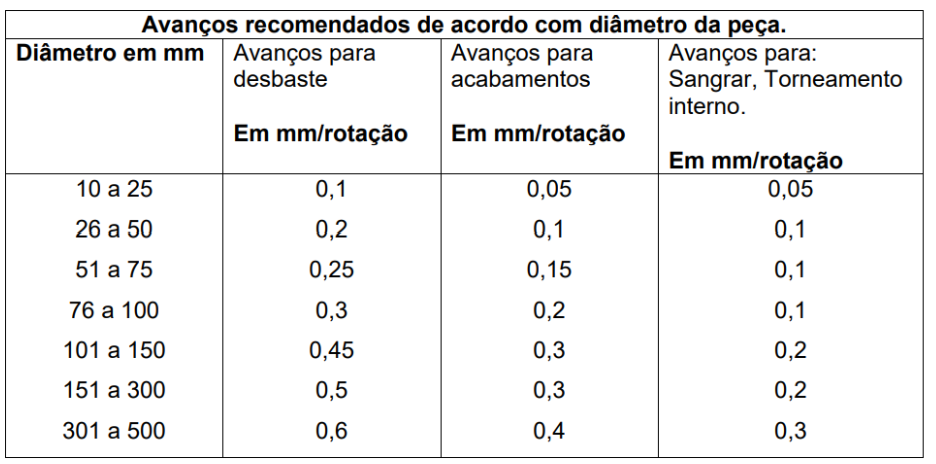
\includegraphics[width=0.7\linewidth]{images/avanco.png}
    \caption{Avaços recomendados de acordo com o diâmetro da peça.}
    \label{fig:enter-label}
\end{figure}

Para o caso do Nylon 6.0, os fabricantes recomendam um avanço de corte de 0,5 mm/rotação para operações de desbaste e 0,05 mm/rotação para operações de acabamento. Essas recomendações visam otimizar a qualidade do corte e a durabilidade da ferramenta, garantindo um bom equilíbrio entre eficiência e precisão durante o processo de usinagem.
\chapter{Estudo das soluções}

\section{Parâmetros avaliados}
Durante o desenvolvimento do projeto, serão analisadas diferentes topologias e soluções para maximizar o desempenho da máquina, considerando parâmetros como frequência natural, rigidez, consumo de materiais e velocidade máxima.

\subsection{Ergonomia}
A máquina foi projetada para facilitar o acesso aos seus componentes e o ajuste manual, quando necessário, considerando a segurança e o conforto do operador.


\subsection{Frequência Natural das Soluções}
O primeiro passo para verificar se a frequência natural de uma máquina está assumindo um valor coerente com a aplicação é comparando-a com a frequência de operação dela. Dessa forma, utilizando uma frequência de operação de 30 MHz --- proveniente dos motores e definida nas especificações de projeto, é preciso garantir que a frequência natural de vibração da solução seja maior que essa. 


Dada a complexidade da estrutura detalhada e da definição de uma equação do movimento que poderia ser proveniente da situação real das guias e das mesas, será utilizado um modelo de simplificação, com algumas hipóteses assumidas. O livro \cite{blevins2001formulas} foi utilizado como base para definição desse modelo estrutural para este cálculo. Assim, a versão simplificada do elemento crítico vibrante --- guia e mesa --- foi considerada como uma barra esbelta com uma massa apoiada no centro. Duas alterativas foram consideradas, representadas na Fig. \ref{fig:blevins-models}.

\begin{figure}[h]
    \centering
    \begin{subfigure}{0.45\textwidth}
         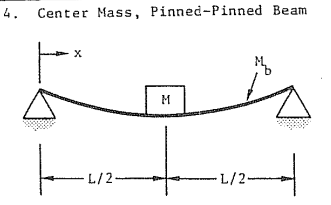
\includegraphics[width=\textwidth]{images/frequencia/center-mass-pinned-pinned.png}
         \caption{Viga bi-apoaiada}
    \end{subfigure}
    \begin{subfigure}{0.45\textwidth}
         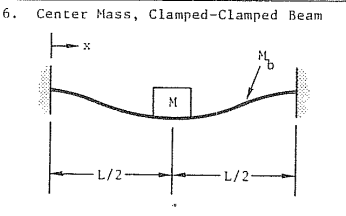
\includegraphics[width=\textwidth]{images/frequencia/center-mass-clamped-clamped.png}
         \caption{Viga bi-engastada}
    \end{subfigure}
    \caption{Modelos de viga esbelta com massa central. Fonte: \cite{blevins2001formulas}}
    \label{fig:blevins-models}
\end{figure}

Para o modelo representado em \ref{fig:blevins-models}(a), a frequência natural pode ser sintetizada pela Eq. \ref{eq:pinned-pinned}, enquanto o modelo em \ref{fig:blevins-models}(b) pela Eq. \ref{eq:clamped-clamped}.

\begin{equation}
\frac{2}{\pi}\left[\frac{3EI}{L^3 (M+0.49M_b)}\right]^{1/2}
\label{eq:pinned-pinned}
\end{equation}

\begin{equation}
\frac{4}{\pi}\left[\frac{3EI}{L^3 (M+0.37M_b)}\right]^{1/2}
\label{eq:clamped-clamped}
\end{equation}

Considerando o pior caso, em que a frequência natural de vibração é menor e, pontanto, mais próxima da frequência mínima limitada pelas especificações do projeto, foi selecionado o modelo da Eq. \ref{eq:pinned-pinned}: a viga bi-apoiada. 

Uma vez selecionado o modelo, é possível estudar a expressão para que sejam especificados os parâmetros utilizados. Destrinchando-os, é preciso conhecer propriedades mecânicas, esturturais e geométricas dos elementos da composição --- guias e a massa móvel:
\begin{itemize}
    \item  E --- módulo de elasticidade do perfil 
    \item I --- segundo momento de inércia do perfil quando uma carga é aplicada e ha deflexão
    \item L --- comprimento do perfil 
    \item M --- massa móvel posicionada no centro do perfil
    \item $M_b$ --- massa dos perfis/guias
\end{itemize}

Adicionalmente, é possível detalhar o momento de inércia  e a massa móvel, definindo-os respectivamente a partir das Eqs. \ref{eq:inertia} e \ref{eq:movel}. O momento de inércia é como o momento de inércia a flexão para duas barras cilíndricas, no caso do eixo das guias. Como a seção é formada for duas barras, deve-se multiplicar o valor de $I$ por dois. Vale ressaltar que esse cálculo pode ser aplicado para as soluções convencionais onde a seção mais propensa a vibração por flexão é a das guias lineares. Posteriormente, na análise de cada uma das soluções, são propostos cálculos de momentos de inércia e massas móveis específicas para cade um dos modelos.  

\begin{equation}
 I = \frac{\pi R^4}{4} 
\label{eq:inertia}
\end{equation}


\begin{dmath}
    M_{\text{móvel}} = (\text{Massa da mesa deslizante})\times 2 + \text{Massa dos perfis da mesa superior} + \text{Massa do porta ferramenta}
\label{eq:movel}
\end{dmath}


A partir dessas expressões, é necessário fornecer o valor de mais parâmetros, sendo eles:
\begin{itemize}
    \item R --- raio dos perfis
    \item $\rho$ --- massa específica do material que compõe o perfil e a mesa (nessa aplicação, esse material é aço)
\end{itemize}


Dessa maneira, é possível determinar, baseado no posicionamento e na escolha das mesa deslizantes assim como sua fixação e adição de massas móveis, qual será a frequência crítica de vibração natural. 

Em adição, é também possível determinar outro tipo de frequência natural de vibração, sendo ela a vibração torsional, que pode ocorrer entre as guias e a mesa. Mas, como essa seria menos menos crítica em relação á frequência de operação, não será limitante para este projeto. 

% de aço = 200 ∗ 109P a
% • L : Comprimento do perfil = 430 ∗ 10−3m
% • Lmesa4 : Comprimento do perfil = 280 ∗ 10−3m
% • R : Raio dos perfis = 10 ∗ 10−3m
% • ρ : massa espec´ıfica a¸co = 7870kg/m3
% • Mb : Massa dos perfis = 2.13kg
% • M : Massa m´ovel = 10.5kg
% • d : distˆancia at´e o eixo = 36 ∗ 10−3m




%% maior rigidez e a da torre -> precisamos determinar a rigidez dele 




%% Frequencia torsional 




% A frequência máxima que vai ser atingida por nossa máquina é 30Hz.(Motores)
% Considerando a rigidez das estruturas das soluções apresentadas, pode-se constatar que os suportes com perfil quadrado em aço de 100mm e 80 mm apresentam um momento de inércia superior ao do perfil da barra delgada da mesa deslizante número 3 que possui 430 mm de comprimento e dois perfis cilíndricos de 20 mm de diâmetro, com um momento de inércia inferior.
% Dessa forma, calculou-se a frequência natural para a mesa deslizante 3 considerando os suportes apresentados nas soluções, biapoiados, e uma massa concentrada no meio dos perfis cilíndricos que corresponde a mesa deslizante de
% número 4, 280 mm, o porta-ferramenta, motor de passo e demais chapas de aço.



\subsection{Rigidez (Loop Estrutural)}
A rigidez estrutural foi analisada para minimizar deformações durante a operação, garantindo precisão e acurácia nas usinagens. O material mole impacta a rigidez.

%%%%%%%%%%%%%%%%%%%%%%%%%%%%%%%%%%%%%%%%%%%%%%%%%%%%%%%%%%%%%%%%


\section{Solução 1}
\begin{figure}[h!]
    \centering
    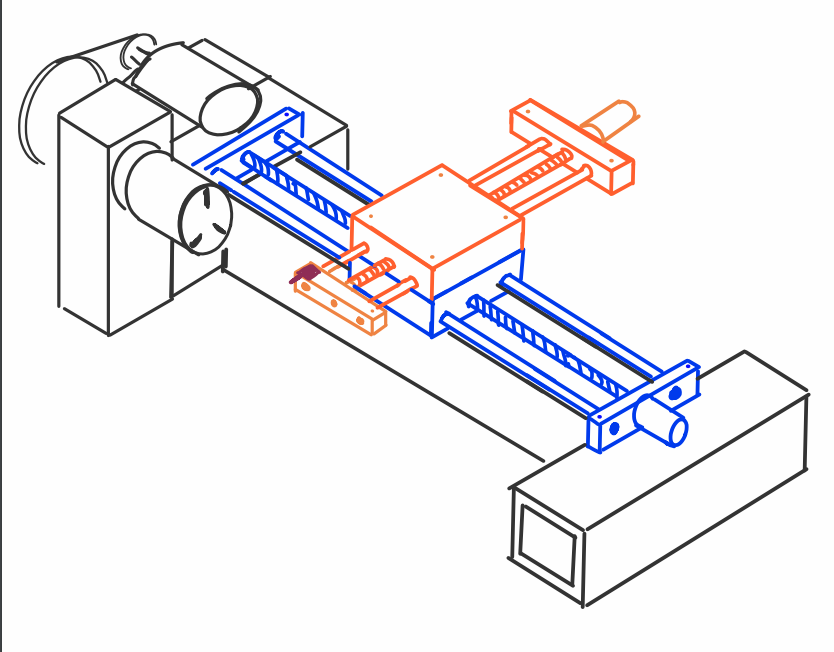
\includegraphics[width=0.7\linewidth]{images/sol1.png}
    \caption{Esboço manual da primeira solução. Fonte: Autor.}
    \label{fig:enter-label}
\end{figure}

\subsection{Peso}

Considerando 3 perfis de 100mmx100mm e tendo como base a estimativa de dimensão: \\
\begin{itemize}
    \item 860mm de comprimento: 8,3kg
    \item 400mm de largura: 3,9kg
    \item 270mm de altura: 2,6kg
\end{itemize}

Com uma chapa de aço 3,2mm entre as mesas considerera-se 290mm de comprimento e 150mm de largura, dimensões suficientes para fixação da guia.  \\
Peso: 0,824 kg \\

Peso extra relacionado a solução 2: 15,7kg \\

\textbf{Peso total:} 40,9kg


\section{Solução 2}

\begin{figure}[h!]
    \centering
    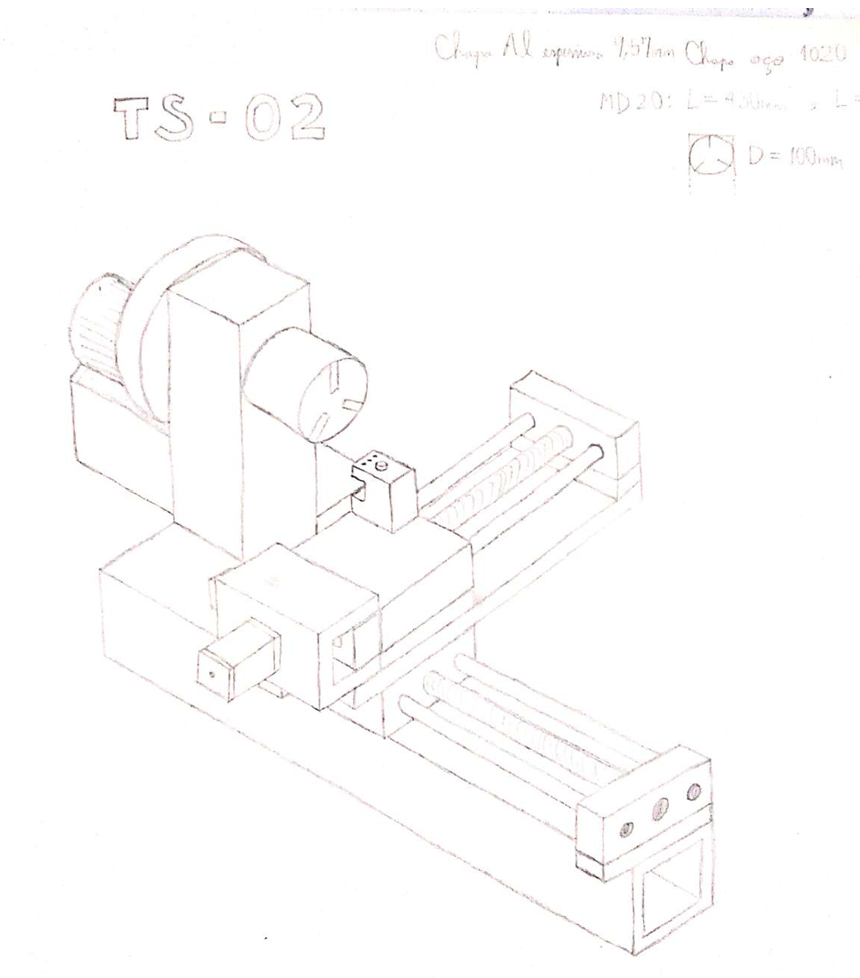
\includegraphics[width=0.7\linewidth]{images/sol2.png}
    \caption{Esboço manual da segunda solução. Fonte: Autor.}
    \label{fig:enter-label}
\end{figure}

\subsection{Peso} 


\section{Solução 3}
\begin{figure}[h!]
    \centering
    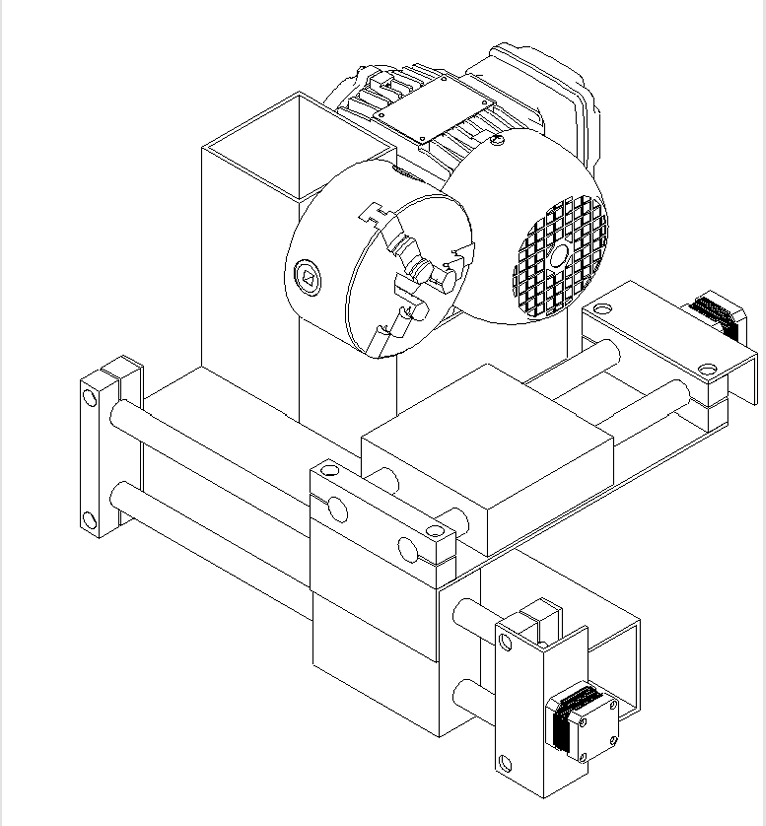
\includegraphics[width=0.7\linewidth]{images/sol3.png}
    \caption{Esboço da terceira solução. Fonte: Autor.}
    \label{fig:enter-label}
\end{figure}

\subsection{Peso}

\begin{itemize}
    \item 2x chapas fixação eixo Z: 0.126 kg
    \item 2x placa motor de passo: 0.586 kg
    \item Eixo árvore: 2.54 kg
    \item Eixo Z : 3.473 kg
    \item Placa mesa de cima : 1.181 kg
    \item Chapa do motor: 0.372 kg 
    \item Base do motor : 1.702 kg
    \item Porta ferramentas: 0.37 kg
\end{itemize}

\textbf{Peso total: }10.35 kg



\section{Matriz de Decisão}

\begin{table}[h]
    \centering
    \begin{tabular}{|c|c|c|c|c|c|c|c|} \hline 
        \multicolumn{2}{|c|}{}& \multicolumn{2}{|c|}{\textbf{Solução 1}} & \multicolumn{2}{|c|}{\textbf{Solução 2}} & \multicolumn{2}{|c|}{\textbf{Solução 3}} \\ \hline  \textbf{Critério}&  \textbf{Peso}& \textbf{Nota} & \textbf{PxN} & \textbf{Nota} & \textbf{PxN} & \textbf{Nota} & \textbf{PxN} \\ \hline  
        Peso & 3 & 3& 9& 5& 15& 3& 9
\\ \hline  
        Rigidez & 7 & 5& 35& 5& 35& 3& 21
\\ \hline  
        Frequência natural & 5 & 3& 15& 5& 25& 1& 5
\\ \hline  
        Velocidade e acelerações & 6 & 3& 18& 5& 30& 3& 18
\\ \hline  
        Erro de Abbe & 3 & 3& 9& 5& 15& 1& 3
\\ \hline  
        Facilidade de montagem & 2 & 3& 6& 5& 10& 1& 2
\\ \hline  
        Facilidade de manufatura & 1 & 3& 3& 5& 5& 3& 3
\\ \hline  
        Segurança do operador & 4 & 1& 4& 5& 20& 5& 20\\ \hline  
 \multicolumn{2}{|c|}{Média Ponderada}& \multicolumn{2}{|c|}{3,35}& \multicolumn{2}{|c|}{4,74}& \multicolumn{2}{|c|}{2,35}\\ \hline 
    \end{tabular}
    \caption{Matriz de decisão entre as soluções propostas.}
    \label{tab:comparativa}
\end{table}

\subsection{justificativa das notas atribídas}

Para todos os critérios, as notas variam de 1 a 5 e procura-se atribuir apenas notas ímpares para as soluções de maneira que haja distanciamento significativo entre as notas medias ponderadas, possibilitando a escolha da solução. 

\begin{itemize}
    \item Peso
    
    Tanto a solução 1 quanto a 3 possuem uma chapa que une a mesa superior à mesa inferior. Por isso, receberam notas menores do que a solução 2. Além disso, o peso adicionado por essa chapa é igual em ambos os casos e não é tão significativo quando comparado ao peso total da máquina para justificar a atribuição de uma nota "1" para as soluções. 
    
    \item Rigidez
    
    A solução 1 e 2 receberam nota máxima nesse quesito, pois é possível identificar que o material a ser uninado seria o ponto mais fraco do laço estrutural. Já para a solução 3 foi atribuída uma nota menor, pois como a ferramenta estaria fixada na ponta da mesa em balanço, a mesa poderia sofrer deformações que afetassem a rigidez da solução.
    
    \item Frequência natural
    
    Dados os modelos de uma viga bi-apoiada para as soluções 1 e 2, e de uma viga com uma das extremidades engastada e a outra em balanço para a solução 3, foram calculadas as frequências naturais de oscilações da estrutura composta pelas guias e mesa deslizantes superiores ads soluções. Assim, as notas foram atribuidas de maneira diretamente proporcional à frequência obtida.

    
    \begin{table}
        \centering
        \begin{tabular}{|c|c|c|c|} \hline 
             Solução&  Frequência [Hz]&  Modo& Nota\\ \hline 
             1&  98&  Flexão& 3\\ \hline 
 2& 102& Flexão&5\\ \hline 
             3&  53&  Flexão& 1\\ \hline
        \end{tabular}
        \caption{Freqências e notas da soluções}
        \label{tab:freq_not}
    \end{table}
    
    \item Velocidade e acelerações
    Como as soluções 1 e 3 possuem maior massa móvel que a 1, foram obtidas para elas acelerações e velocidades máximas menores que para solução 2. assim, elas receberam notas menores
    
    \item Erro de Abbe
    
    O Erro de Abbe foi considerado ao analisar a altura da ferramenta em relação ao seu ponto de fixação na quia ou mesa. Essa metodologia foi escolhida pois quanto maior é o porta ferramentas, maior é a deformação gerada nele por conta das forças de usinagem e maior o erro de Abbe.
    
    \item Facilidade de montagem
    
    Esse critério foi analisado contando o número de peças necessárias para formar a solução. Além disso, a solução 3 recebeu uma nota menor que a 1, apesar de ter o mesmo numero de peças, por ter uma das extremidades em balanço, o que causaria uma dificuldade para alinhamento das estruturas.
    
    \item Facilidade de manufatura
    
    Esse critério foi analisado contando o número de peças necessárias para formar a solução. A solução com menor número de peças recebeu a maior nota.
    
    \item Segurança do operador
    
    As soluções 1 e 2 receberam as mesmas notas, mas a solução 3 recebeu uma nota menor por conta da possibilidade de acidentes que podem ser causados pelas vibrações e deformações excessivas em sua extremidade livre.
    
\end{itemize}

\chapter{Projeto}

(dar um nome melhor pra seção de solução escolhida)


\section{Esquema Elétrico}
Na área de atuadores, foi realizada uma análise do esquema elétrico fornecido pelo professor. A partir disso, verificaram-se as conexões da porta paralela, assim como os componentes e conexões utilizados. Abaixo estão as imagens do esquema original (Fig. \ref{fig:prof_schematic}) e do desenvolvido no KiCad (Fig. \ref{fig:kicad_schematic}).

\begin{figure}[H]
    \centering
    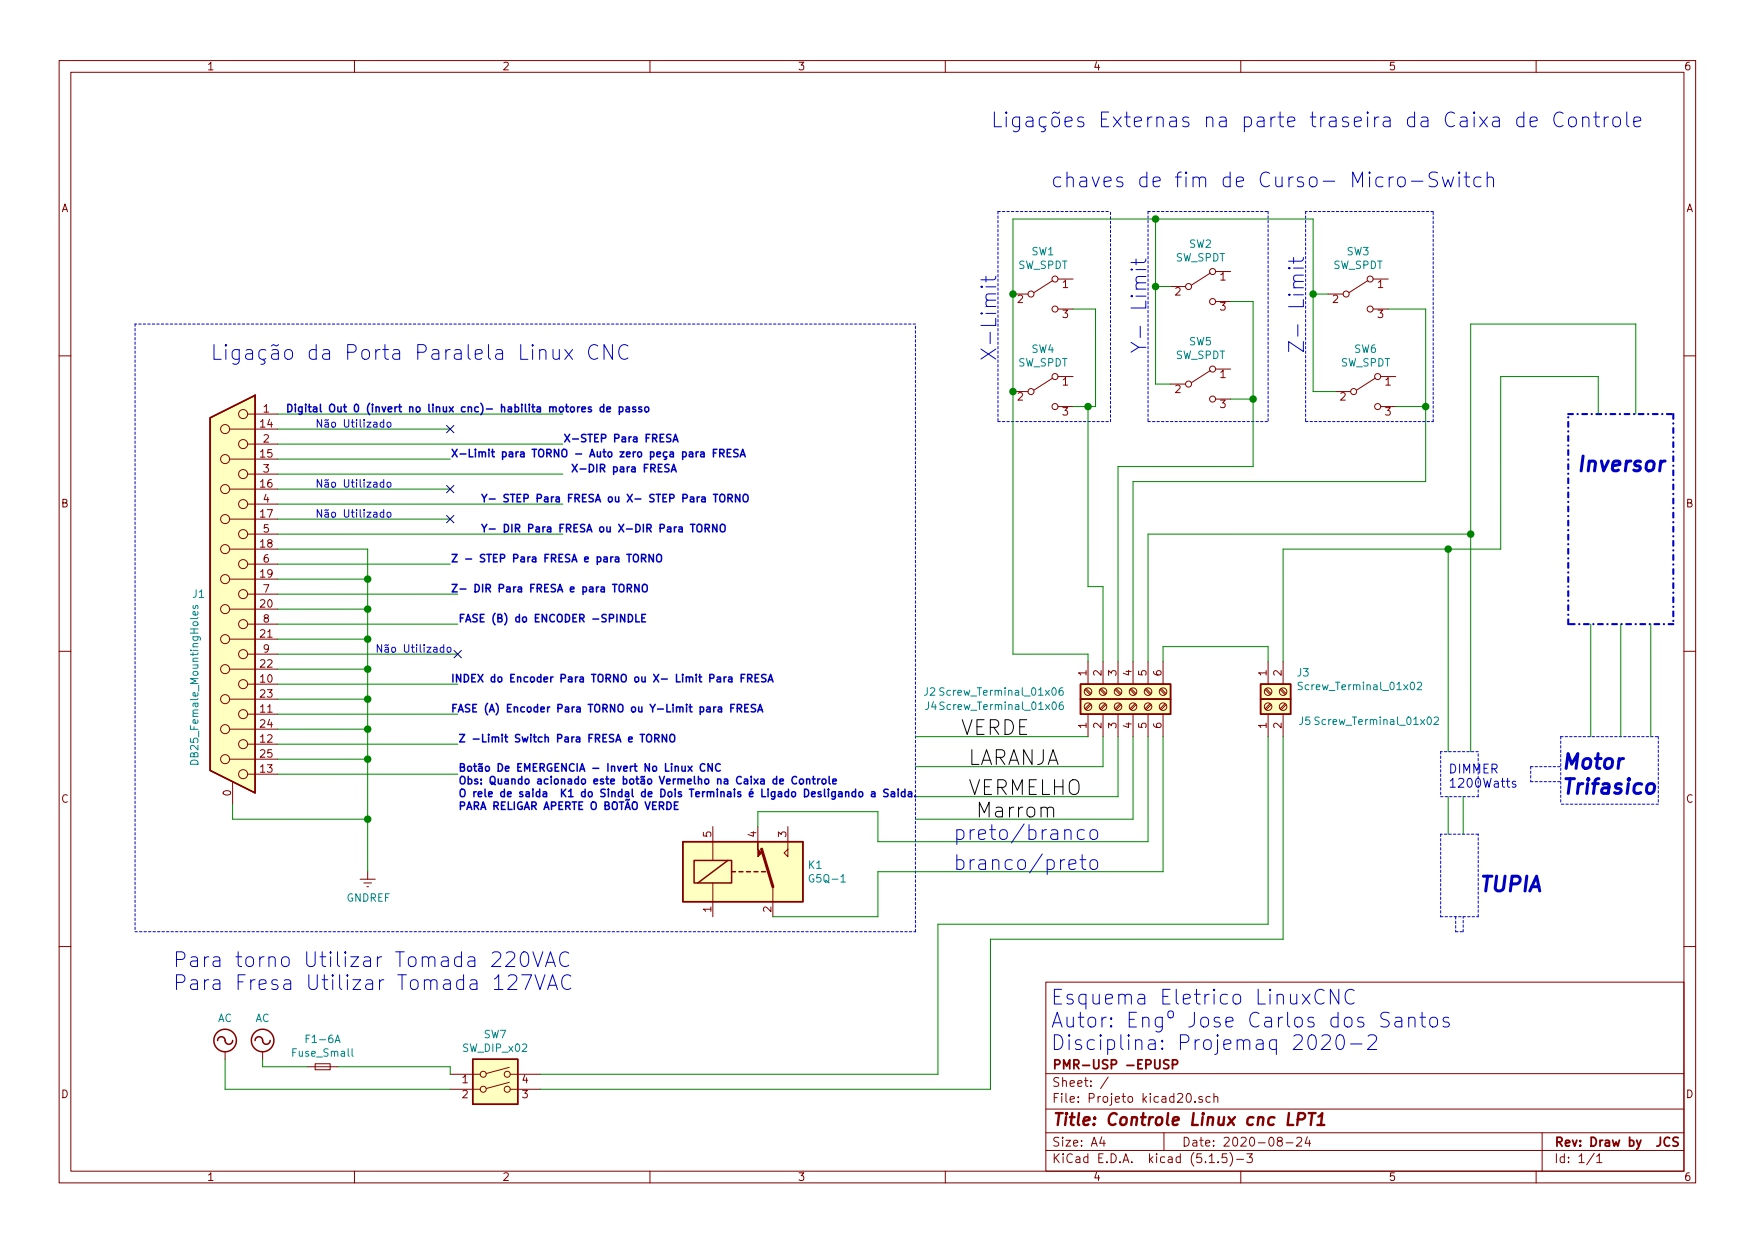
\includegraphics[width=\textwidth]{images/kicad-prof.jpg}
    \caption{Esquema elétrico fornecido pelo professor}
    \label{fig:prof_schematic}
\end{figure}

\begin{figure}[H]
    \centering
    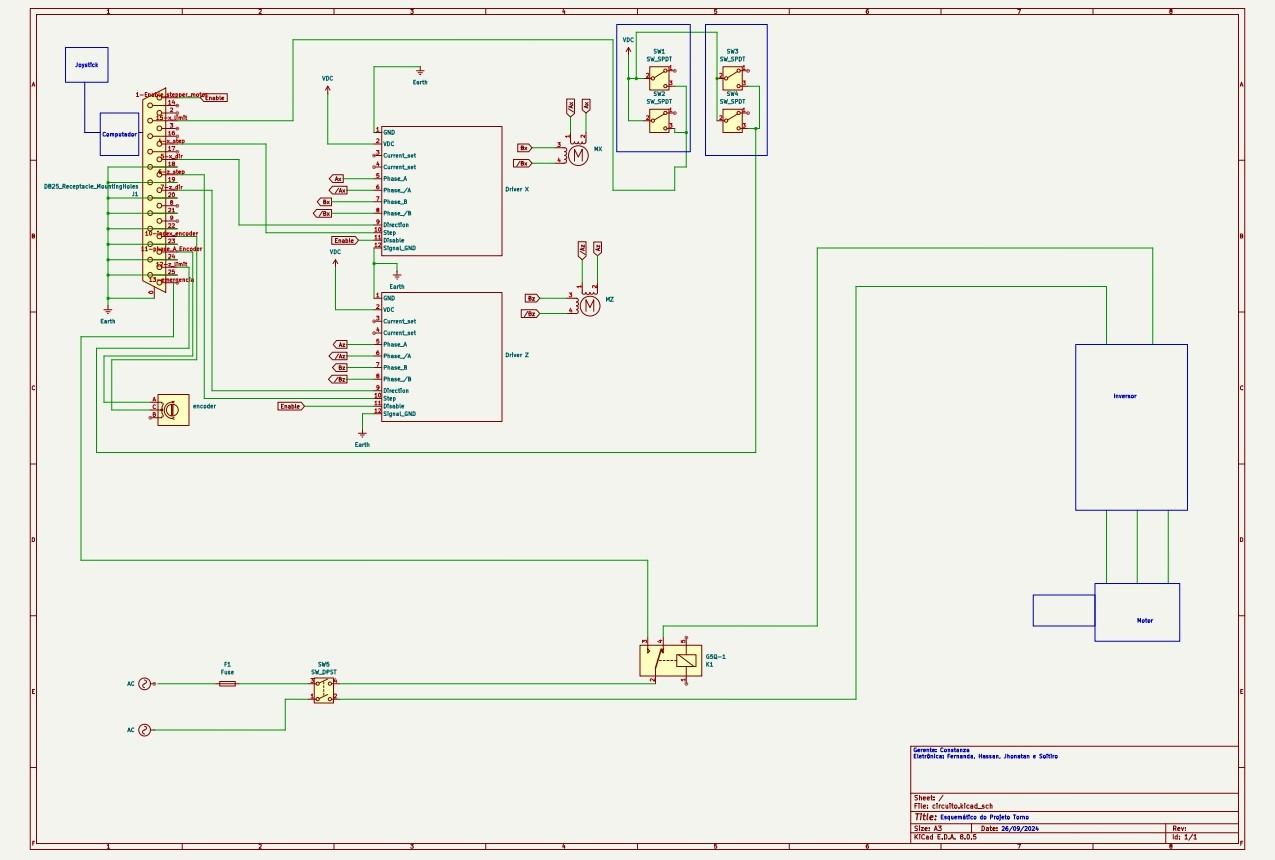
\includegraphics[width=\textwidth]{images/nosso-kicad.jpg}
    \caption{Esquema elétrico desenvolvido no KiCad}
    \label{fig:kicad_schematic}
\end{figure}

Algumas observações importantes incluem o fato de que o driver utilizado não estava disponível na biblioteca do KiCad, o que tornou necessário criá-lo seguindo as especificações técnicas de seu datasheet. No caso do encoder, foram consideradas apenas duas fases: a fase A e o index.

Para evitar "poluição visual", adotaram-se etiquetas para referenciar as conexões. Para o inversor e o motor, foi feito um esboço simplificado dos componentes, já que as suas características específicas não estavam presentes na biblioteca.



\chapter{Programação}

A função da subárea de programação nesse projeto foi desenvolver o CAM e posteriormente o código G de peças que o grupo desejasse usinar, além de preparar o ambiente do LinuxCNC para a execução desse código por meio de configurações e instalações de programas, aspectos que serão discutidos adiante. Além disso, à essa subárea coube o papel de aprender a controlar a máquina manualmente e repassar esse conhecimento aos demais membros do grupo. 

Assim, a programação adequada envolve não apenas o preparo do ambiente (configuração de eixos, homing e seleção de planos de corte)e a criação de código G, mas também a implementação de ferramentas auxiliares, como o uso do qjoypad para mapear comandos do teclado em um Joystick, tornando a operação manual mais intuitiva e, tão importante quanto, a transmissão de conhecimento de operação para todo o grupo.

\section{Configuração feita no Stepconf Wizard}

O aplicativo chamado Stepconf Wizard é a ferramenta mais prática disponível no LinuxCNC para a geração dos arquivos de configuração necessários para a operação da máquina que foi montada. A partir da seleção de parâmetros desejados em sua interface gráfica ele gera automaticamente arquivos de configuração \textit{.hal} que são a camada de abstração entre o hardware da máquina e o software de controle. 

Inicialmente foram escolhidos o nome do projeto, a configuração de eixos (isso definiu a máquina como um torno) e a unidade de comprimento padrão. Além disso, foi escolhido o driver Gecko 201, um driver que foi informado ao grupo por um dos técnicos como sendo o adequado para os motores de passo utilizados.

Para encontrar o máximo atraso entre comandos enviados pela porta paralela (jitter) foi preciso apenas executar um teste de latência enquanto a máquina é submetida a estresse computacional. Para fazer isso basta executar o comando \textbf{latencytest} em um terminal, o que abre um aplicativo que monitora os tempos de resposta e informa o máximo atraso medido. A seguir é mostrada uma imagem dessa configuração inicial:

\begin{figure}[H]
    \begin{center}
        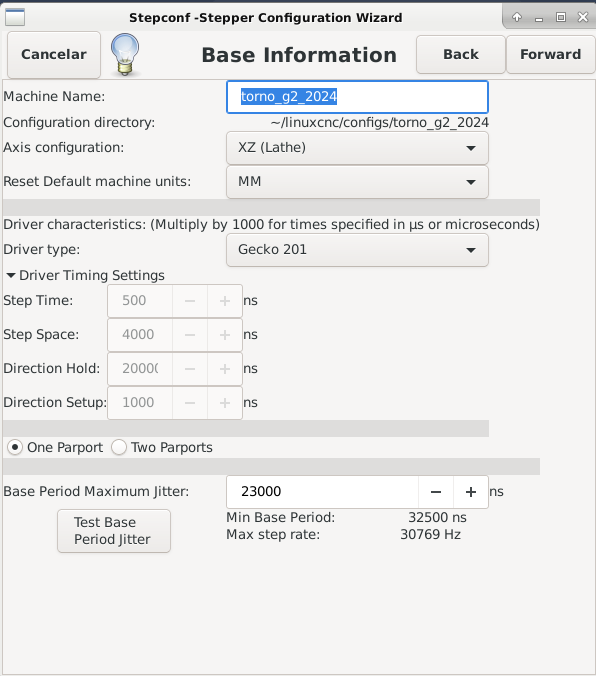
\includegraphics[width=0.95\textwidth]{images/prog/stepconf1.png}
    \end{center}
    \caption{Configuração inicial}\label{step1}
\end{figure}

Para que o LinuxCNC seja capaz de enviar sinais corretos para a caixa de controle a pinagem da porta paralela é definida em seguida. Essa pinagem foi disponibilizada para os alunos no moodle no inicio do curso e já foi apresentada anteriormente nesse relatório, porém, devido a peculiaridade da máquina girar seu eixo árvore no sentido anti-horário, a ferramenta foi colada do lado oposto ao usual, o que obrigou o grupo a inverter o sinal do pino que controla a direção do eixo X, de modo que avanços positivos comandados por código G realmente representassem uma aproximação da ferramenta em relação ao material usinado.

\begin{figure}[H]
    \begin{center}
        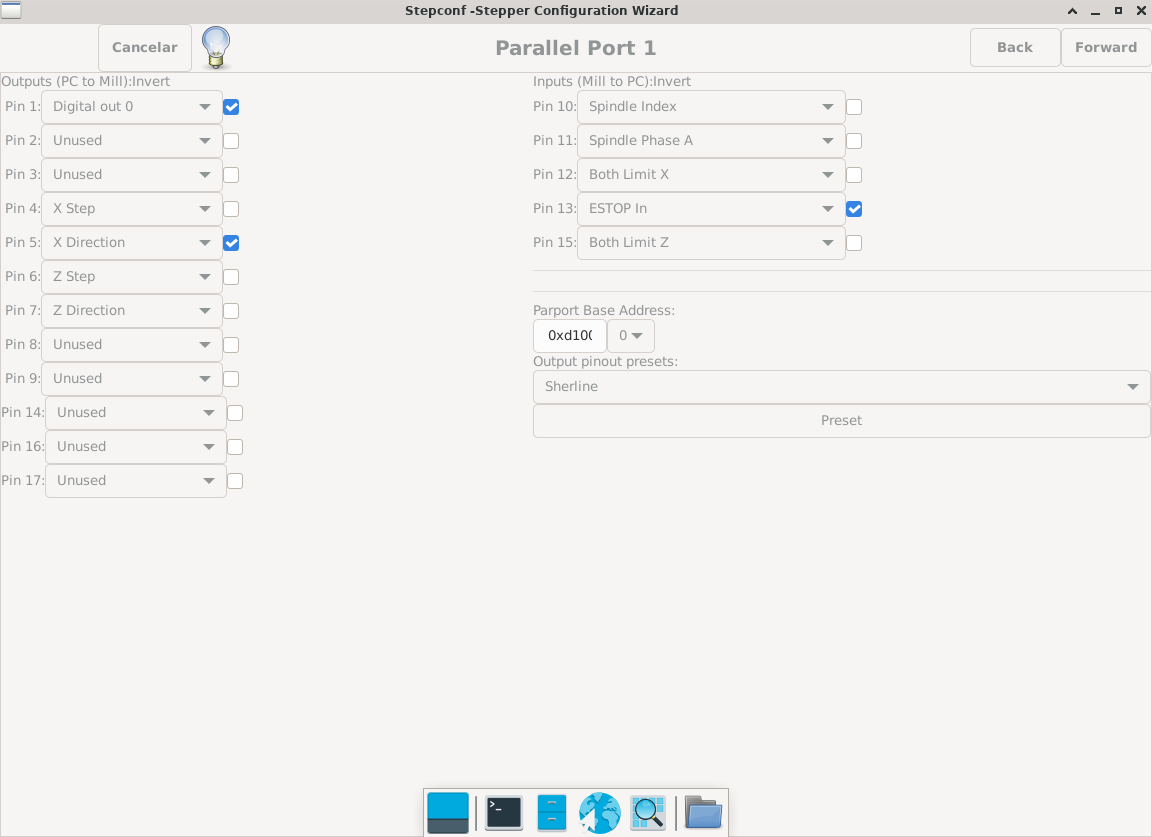
\includegraphics[width=0.95\textwidth]{images/prog/stepconf_config.png}
    \end{center}
    \caption{Configuração dos pinos da porta paralela}\label{pinagem}
\end{figure}

Os parâmetros de usinagem de cada eixo são definidos em seguida, sendo os mais relevantes as velocidades e acelerações máximas (25 mm/s e 750 mm/s, respectivamente) que foram definidos levando em consideração segurança de operação e integridade do equipamento (velocidades e acelerações muito grandes aumentam os riscos e as consequências de erros) e recomendações de técnicos que asseguraram ao grupo que essas configurações (que são o padrão) seriam mais que suficientes para as tarefas à serem executadas. Cabe ainda destacar que ambos os eixos receberam a mesma configuração, e que os seus limites estão definidos como valores muito grandes, uma vez que os verdadeiros limites foram definidos pelas chaves de fim de curso, não havendo assim necessidade de utilizar essa configuração para impor limites de deslocamento.

\begin{figure}[H]
    \begin{center}
        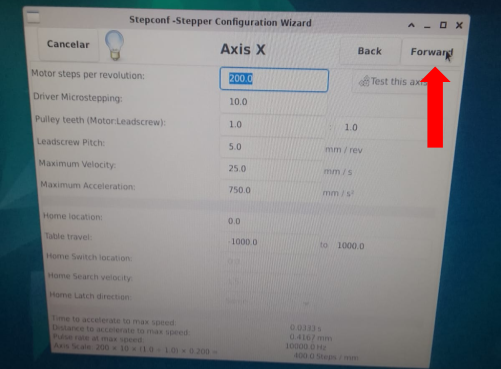
\includegraphics[width=0.95\textwidth]{images/Eletrica/Figura8.png} % lembrar de conseguir uma imagem melhor %
    \end{center}
    \caption{Configuração de um dos eixos}\label{eixos}
\end{figure}

\section{Configuração do controle manual}

Como requerimento de projeto foi pedido que o grupo mapeasse comandos do teclado que controlam os aspectos de controle manual da máquina no LinuxCNC para um Joystick, por meio de algum programa, de modo a facilitar o controle manual da máquina. Para realizar esse mapeamento, o grupo utilizou um fork do programa qjoypad, disponível na snapstore (problemas com a instalação serão tratados mais adiante na seção de desafios encontrados).
Foram mapeados para o Joystick os seguintes comandos:

\begin{itemize}
    \item Direita (d-pad direito, analógico) 
    \item Esquerda (d-pad esquerdo, analógico)
    \item Cima (d-pad acima, analógico)
    \item Baixo (d-pad abaixo, analógico)
    \item Aumentar velocidade (R1) 
    \item Diminuir velocidade (L1)
    \item Selecionar eixo X (L2)
    \item Selecionar eixo Z (R2)
    \item Homing do eixo selecionado (L3, R3, botão 3)
\end{itemize}

Abaixo, imagens das configurações feitas:

\begin{figure}[H]
    \begin{center}
        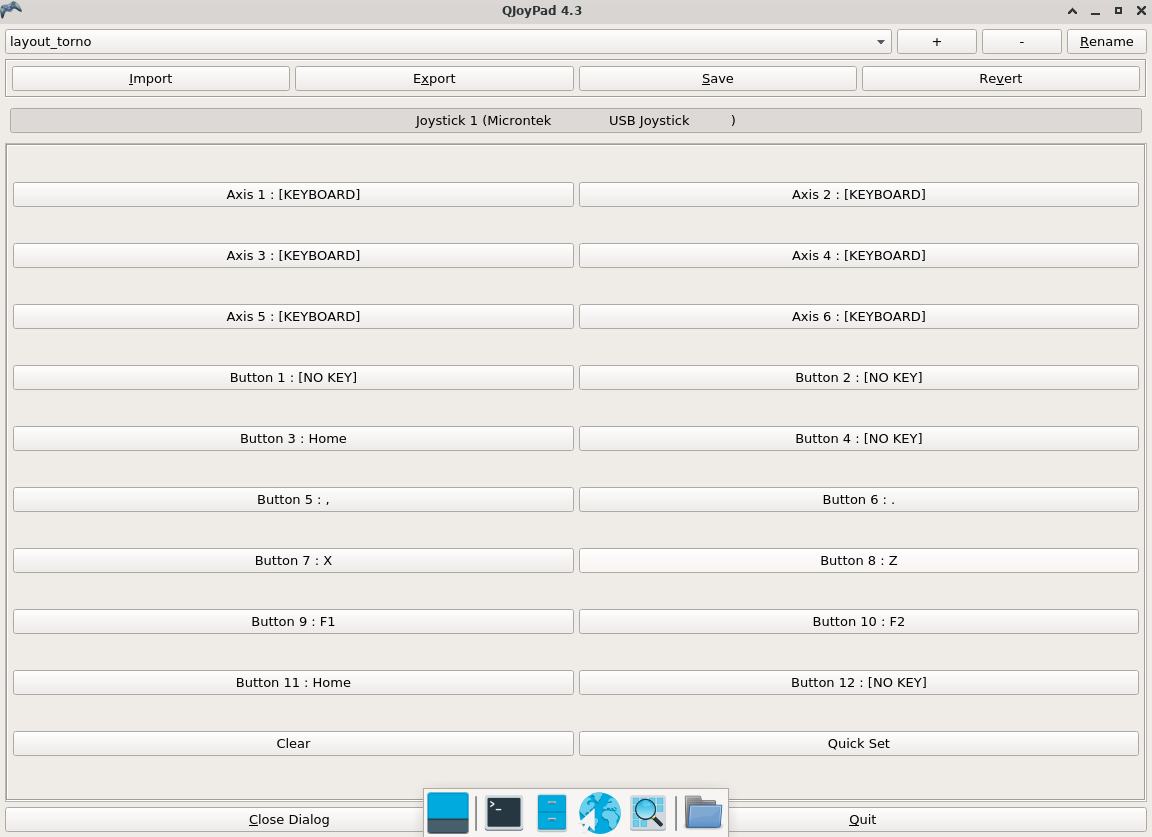
\includegraphics[width=0.95\textwidth]{images/prog/qjoypad_config.png}
    \end{center}
    \caption{Mapeamento feito no qjoypad}\label{qjoypad}
\end{figure}


\begin{figure}[H]
    \begin{center}
        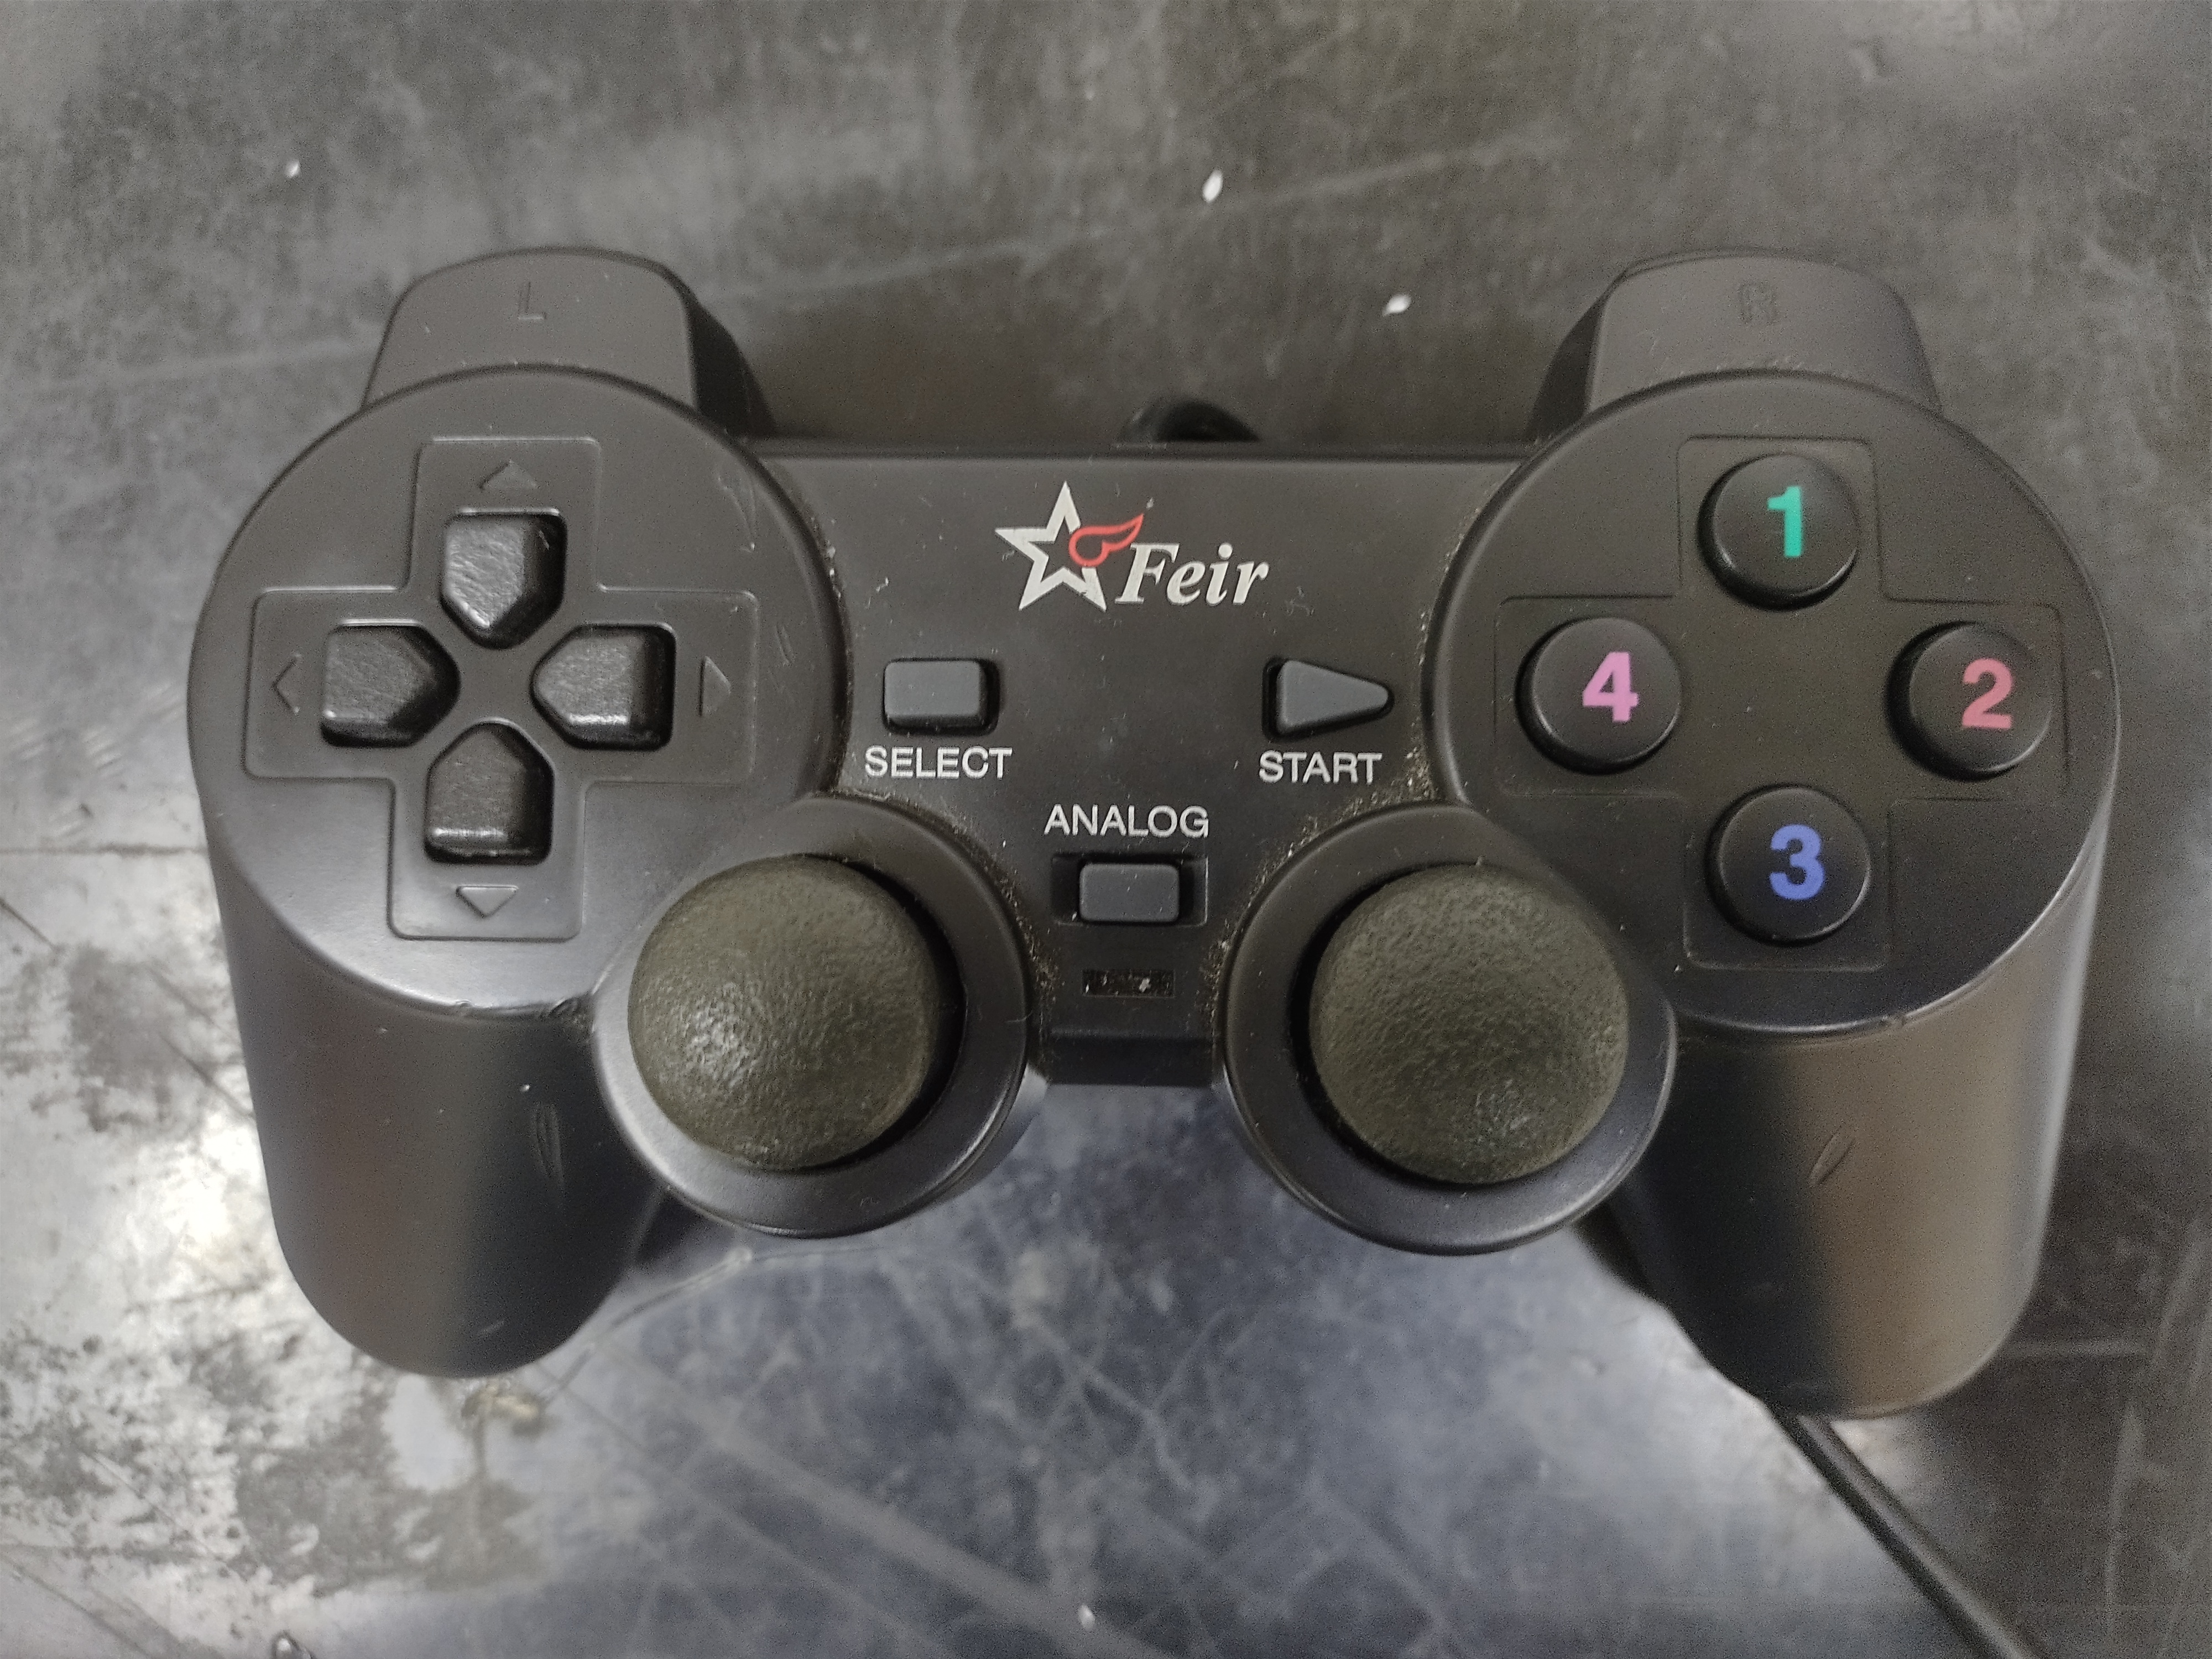
\includegraphics[width=0.95\textwidth]{images/prog/fotocontrole.png}
    \end{center}
    \caption{Comandos mapeados indicados no Joystick}\label{controle_joy}
\end{figure}

Cabe ressaltar que, para inicializar o qjoypad, e por consequência habilitar o controle manual no Joystick, é preciso executar o comando qjoypad no terminal. 

\section{Códigos G}
\subsection{Geração de códigos G}

A geração de códigos G se deu através da utilização da utilização do software Inventor CAM. A partir de um modelo também feito no Inventor, foram selecionados diversos parâmetros de usinagem de modo que uma simulação fidedigna de usinagem pudesse ser gerada. Os parâmetros mais relevantes estão listados a seguir: 

\begin{itemize}
    \item Tipo de ferramenta
    \item Velocidade de corte
    \item Velocidade de rotação
    \item Profundidade de corte máxima
    \item Fronteiras de corte
    \item Estratégia de corte
\end{itemize}

Como exemplo do que está descrito acima, seguem imagens da produção do CAM da peça final:

\begin{figure}[H]
    \begin{center}
        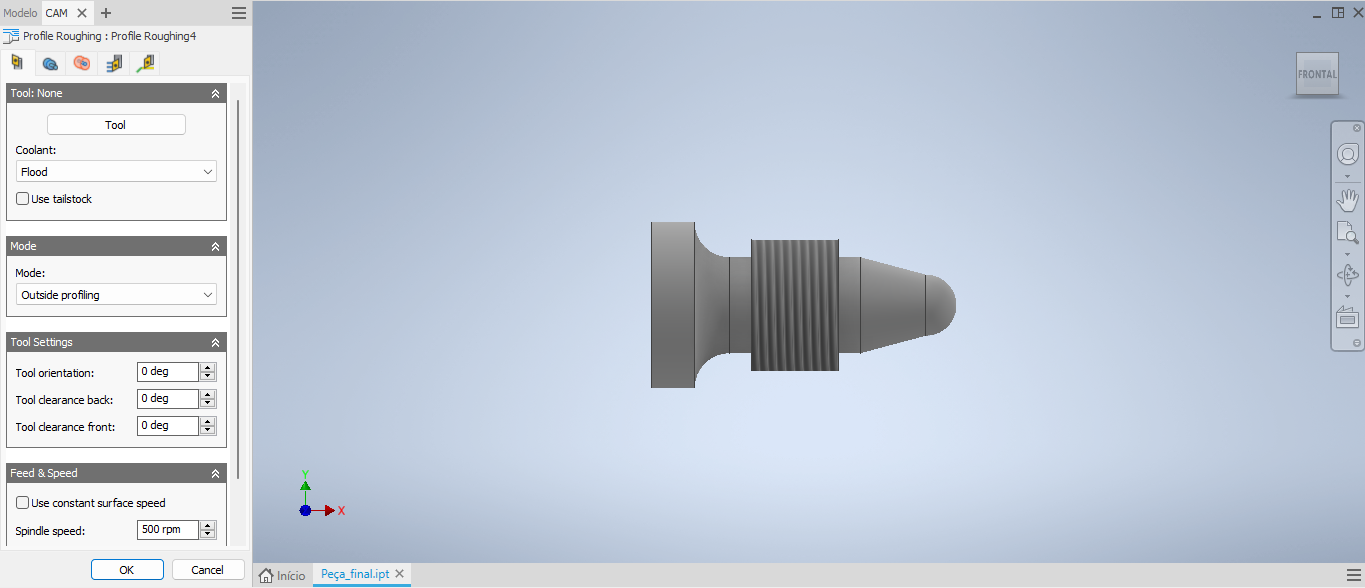
\includegraphics[width=0.95\textwidth]{images/prog/cam.png}
    \end{center}
    \caption{Interface onde são inseridas informações}\label{inicio_cam}
\end{figure}

\begin{figure}[H]
    \begin{center}
        \includegraphics[width=0.95\textwidth]{images/prog/cam_peça.png}
    \end{center}
    \caption{Caminho de desbaste gerado para a peça final}\label{cam_desbaste}
\end{figure}

\subsection{Tratamento do código G gerado}

Como os códigos gerados automaticamente não foram muito extensos, o grupo de programação lançou mão de revisões manuais para correção de eventuais erros. Erros comuns como o programa gerar códigos utilizando o código G32 (não suportado pelo LinuxCNC) ou utilizar coordenadas com nomenclatura U e W ao invés de X e Z podem ser facilmente resolvidos com o uso de uma função de encontrar e substituir, muito comum em editores de texto modernos. 

Para o ajuste de parâmetros de usinagem pontuais, como por exemplo velocidades, adição ou remoção de pausas para troca de ferramenta, e profundidades de corte, também se buscou usar de edições manuais no código, evitando a modificação de simulações no CAM ao máximo, apenas por uma questão de praticidade. Para tanto, o grupo instalou na máquina designada o editor Vscode, jundo de uma extensão que destaca sintaxe de código G.

\begin{figure}[H]
    \begin{center}
        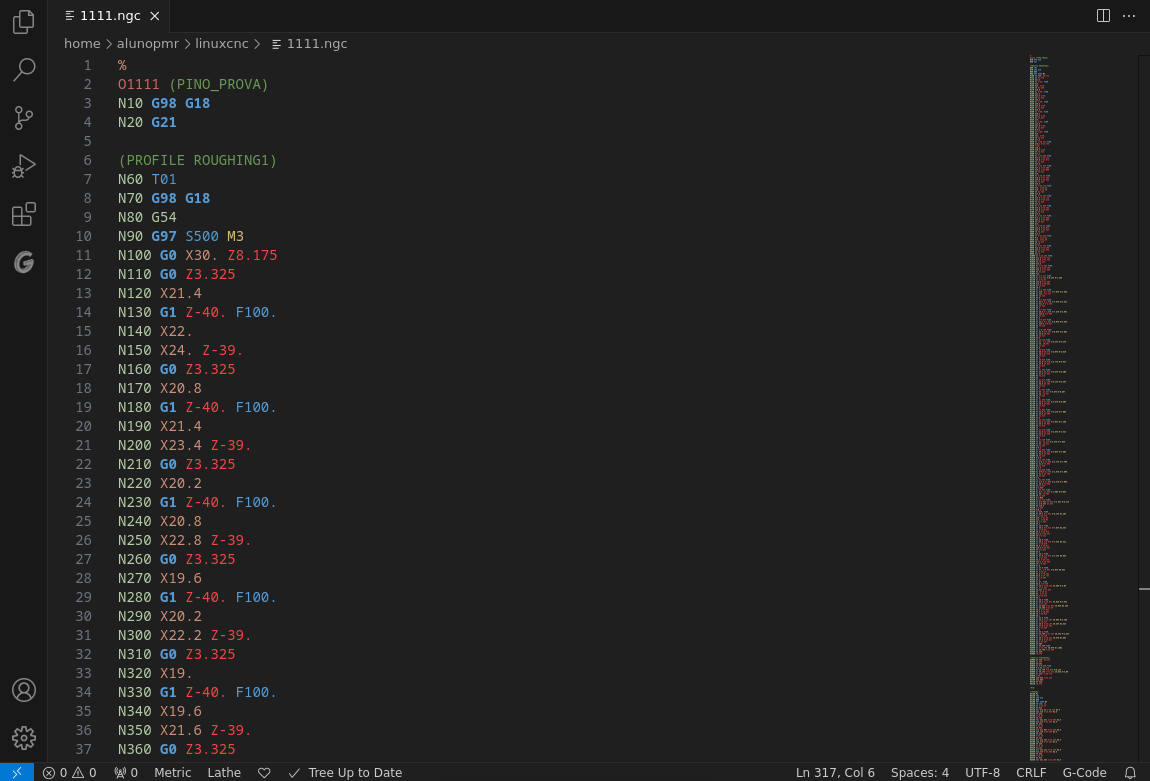
\includegraphics[width=0.95\textwidth]{images/prog/codigo_g.png}
    \end{center}
    \caption{Vscode com um código sendo editado}\label{code}
\end{figure}

Assim como o qjoypad, a instalação do Vscode foi feita através da instalação de um snap da snapstore.

\section{Procedimento de usinagem}

Idealmente, o grupo se reuniria para que os membros que soubessem operar a máquina repassassem esse conhecimento para os demais, o que de fato foi feito diversas vezes. Dito isso, o grupo de programação decidiu criar um manual de manuseio da máquina, de modo que todos pudessem estudar a máquina no horário que pudessem, evitando assim que a absência de membros do grupo por motivos adversos prejudicasse os demais. O procedimento descrito nos subtópicos a seguir é um resumo desse manual.

\subsection{Tratamento Inicial da Peça: Desbaste e Faceamento}

Antes de executar códigos G complexos, é essencial preparar a peça para a usinagem por meio de operações de desbaste e faceamento. Essas etapas garantem superfícies regulares e dimensões iniciais adequadas para a peça.

\subsection{Posicionamento Manual da Ferramenta}

Para ambas as operações, o operador deve posicionar a ferramenta manualmente:

\begin{itemize}
    \item Utilize o controle manual (Joystick ou teclado) para aproximar a ferramenta da peça.
    \item Ajuste a velocidade de avanço (Jog Speed) para um valor seguro, geralmente entre 20 e 50 mm/s.
    \item Posicione a ferramenta próximo à superfície da peça, garantindo uma pequena folga para evitar colisões.
\end{itemize}

\subsubsection{Desbaste}

O desbaste remove o excesso de material da superfície externa da peça, garantindo uniformidade ao diâmetro. Procedimentos principais:

\begin{itemize}
    \item Mova a ferramenta lateralmente ao longo do eixo Z, mantendo o eixo X fixo.
    \item Realize cortes sucessivos, reduzindo gradualmente o diâmetro até atingir o valor desejado.
    \item Monitore visualmente o processo e ajuste a velocidade de avanço conforme necessário.
\end{itemize}

\subsubsection{Faceamento}

O faceamento nivela a face da peça, removendo irregularidades. Etapas:

\begin{itemize}
    \item Posicione a ferramenta próxima à extremidade frontal da peça.
    \item Mova a ferramenta ao longo do eixo X, com o eixo Z fixo.
    \item Realize cortes suaves e uniformes até que toda a face da peça esteja nivelada.
\end{itemize}

Ambas as operações devem ser realizadas com cuidado para evitar colisões e assegurar que a peça esteja firme na placa de fixação.

\subsection{Configuração Inicial do Ambiente de Programação}

Antes de iniciar a programação efetiva do torno, é preciso preparar o ambiente de execução do LinuxCNC. Alguns pontos-chave:

\begin{itemize}
    \item \textbf{Ligação dos dispositivos:} É recomendável que a caixa de controle da máquina esteja ligada e o Joystick conectado antes da inicialização do computador. Isso previne problemas de detecção de periféricos pelo LinuxCNC.
    \item \textbf{Login e Sistema:} Após ligar o computador (com caixa de controle já energizada), efetua-se o login no sistema operacional. 
    \item \textbf{Execução do LinuxCNC:} Com o LinuxCNC aberto, deve-se selecionar a configuração apropriada do torno. Uma vez carregada a interface principal, o usuário pode então dar início à programação e à interação com o ambiente de usinagem.
\end{itemize}

\subsection{Referenciamento (Homing) e Modos de Coordenadas}

Um passo fundamental na etapa de programação é o homing dos eixos (X e Z). Esse processo estabelece a posição de referência absoluta da máquina, conhecida como zero máquina, imprescindível para qualquer subsequente programa em código G. 

Após realizar o homing, o usuário pode definir planos de corte (por exemplo, G54) e zeros de peça, garantindo que o código G seja interpretado corretamente em relação à posição física da ferramenta e do tarugo a ser usinado.

\subsubsection{Definição do Zero Peça}

Definir o zero peça envolve posicionar a ferramenta em contato com o material e, através de recursos do LinuxCNC (como o apalpador), informar ao controlador o deslocamento necessário. Para o eixo Z, posiciona-se a ferramenta na face do tarugo; já para o eixo X, é necessário conhecer o diâmetro do tarugo. Essa informação garante que o código G seja interpretado corretamente, especialmente ao trabalhar em modo de diâmetro (G7).

O correto ajuste do zero peça é determinante para assegurar que o caminho programado no código G resulte em movimentos seguros e precisos, evitando colisões e garantindo o correto posicionamento da ferramenta em relação à geometria desejada.

\subsection{Carregando e Executando Código G}

A programação do torno CNC via LinuxCNC baseia-se na leitura e execução de arquivos com extensão \textit{.ngc}, contendo instruções G-code. Após ajustar o zero peça e conferir se o modo de diâmetro (G7) está ativado quando necessário, o usuário pode abrir o arquivo desejado:

\begin{itemize}
    \item \textbf{Seleção do Programa:} Através da interface gráfica do LinuxCNC, o usuário seleciona o arquivo \textit{.ngc} a ser executado.
    \item \textbf{Pré-visualização:} Antes da execução, o preview mostra o caminho da ferramenta, permitindo checar visualmente se o trajeto faz sentido.
    \item \textbf{Execução:} Ao dar início à execução, o LinuxCNC seguirá as instruções do código G, respeitando parâmetros de avanço, velocidade e comandos de mudança de ferramenta.
\end{itemize}

Durante este processo, é possível ajustar fatores como a velocidade máxima de execução, garantindo maior segurança caso haja incerteza sobre o comportamento do programa.

\section{Desafios encontrados}

Além dos problemas recorrentes e simples de serem solucionados, como por exemplo o ajuste de códigos G (ou até mesmo eventuais modificações em um CAM) além de afiações e ajustes de ferramenta para garantir que o torno produzisse resultados adequados, o grupo de programação deve de superar alguns desafios que merecem destaque. Nos subtópicos a seguir estes desafios serão listados e discutidos.

\subsection{Modo de diâmetro (G07)}

Sem dúvidas esse foi o erro que custou mais tempo do grupo de programação (cerca de uma semana para a solução). Esse erro foi observado pela primeira vez ao se tentar produzir uma peça com um raio esférico na sua ponta, o que gerou uma mensagem de erro que indicava o que aparentemente eram dois raios distintos e conflitantes no código.

\begin{figure}[H]
    \begin{center}
        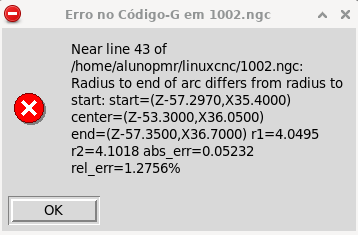
\includegraphics[width=0.95\textwidth]{images/prog/erro_g7.png}
    \end{center}
    \caption{Erro apresentado quando G07 não está ativo}\label{g07}
\end{figure}

O fato de que ninguém para o qual nós apresentamos esse erro pôde identificar erros no código G indicou para o grupo que havia um erro desconhecido ocorrendo no interpretador do LinuxCNC. Como nada do que foi tentado funcionou, a medida de trocar o computador e copiar a configuração de ambiente de outro grupo que teve seu sistema operacional atualizado foi tomada, porém isso não solucionou o problema. 

No fim, o grupo descobriu, ao observar a indicação da posição do eixo X na interface gráfica, que o comportamento padrão do LinuxCNC presente na máquina era de ter o modo de coordenadas em raio ativado, o que é incomum para códigos de usinagem CNC. Assim, a única solução encontrada foi a ativação do código G07 a partir do MDI antes de carregar qualquer código G. 

Além do tempo necessário para finalmente descobrir a causa real do problema, a maior parte do tempo gasto devido a esse erro veio do fato de o grupo ter de configurar o ambiente de execução novamente devido a troca de computador. Além disso, essa troca foi a causa do próximo problema que será discutido. 

\subsection{Instalação do qjoypad}

Inicialmente o programa qjoypad já estava instalado na máquina que o grupo recebeu, de modo que o trabalho de configurar o controle manual se resumiu à apenas mapear os comandos no aplicativo. No entanto, devido a troca de computador e atualização de sistema operacional, o programa teve de ser instalado novamente. 

O processo de instalação do aplicativo original, disponível na Source Forge, é simplesmente a sua compilação a partir dos arquivos fonte. Porém isso não foi possível, pois o sistema operacional recentemente instalado não possuía uma ferramenta de compilação chamada de \textbf{qmake}, a qual tinha um processo de instalação que precisaria de internet para ser viável. 

Já com acesso a internet, por meio de roteamento à partir de telefones móveis, foi constado que a instalação de qualquer pacote seria muito dificultada pois o sistema não tinha nem uma lista dos repositórios remotos padrões do Debian, provavelmente devido ao tipo de instalação feita (totalmente offline). Finalmente ao achar o arquivo de configurações de fontes remotas do Debian, foram adicionadas as seguintes fontes:

\begin{figure}[H]
    \begin{center}
        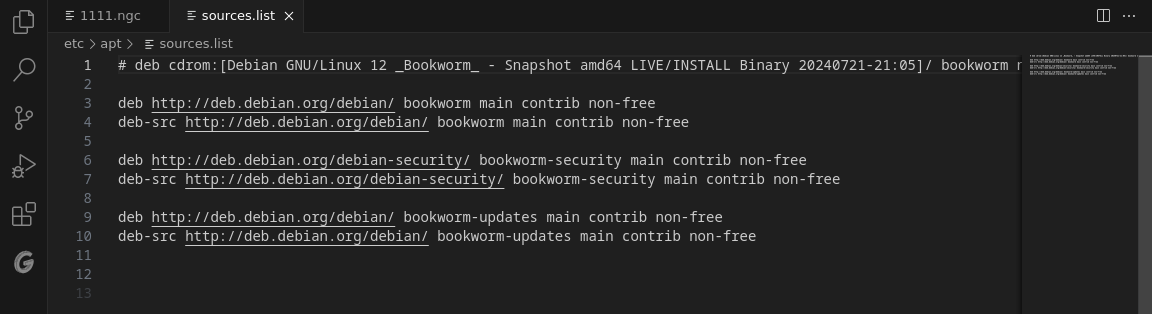
\includegraphics[width=0.95\textwidth]{images/prog/fontes.png}
    \end{center}
    \caption{Repositórios remotos adicionados}\label{fontes}
\end{figure}

Com essas fontes instaladas, foi possível instalar a snapstore e, a partir dela, um snap de um fork mais novo do qjoypad, com as mesmas funcionalidades do original.

\subsection{Reconhecimento de periféricos}

Esse problema se manifesta pelo fato do LinuxCNC instalado na primeira máquina que o grupo recebeu não procurar por periféricos após a inicialização, o que significa que qualquer dispositivo que o grupo quisesse conectar em alguma porta USB, como por exemplo o Joystick ou um pendrive, deveria ser conectado antes da inicialização. Esse problema simplesmente entrou para o procedimento de usinagem como um aviso de conectar tudo antes de ligar o computador. 

Após a troca de computador, no entanto, o LinuxCNC se tornou capaz de reconhecer periféricos conectados após a inicialização, então o problema foi definitivamente resolvido após a atualização.

\chapter{Próximos passos}



\printbibliography

\chapter{Anexos}



\begin{comment}

Procurar livros no \url{https://books.google.com.br/}, lá tem a opção "BiBTeX" com a estrutura já pronta. Caso contrário, seguir uma das seguintes estruturas:

\section{Artigo}

@article{einstein,
    author = "Albert Einstein",
    title = "{Zur Elektrodynamik bewegter K{\"o}rper}. ({German})
    [{On} the electrodynamics of moving bodies]",
    journal = "Annalen der Physik",
    volume = "322",
    number = "10",
    pages = "891--921",
    year = "1905",
    DOI = "http://dx.doi.org/10.1002/andp.19053221004",
    keywords = "physics"}

\cite{einstein}


\section{Livro}

@book{dirac,
    title = {The Principles of Quantum Mechanics},
    author = {Paul Adrien Maurice Dirac},
    isbn = {9780198520115},
    series = {International series of monographs on physics},
    year = {1981},
    publisher = {Clarendon Press},
    keywords = {physics}}

\cite{dirac}
%%%%%%%%%%%%%%%%%%%%%%%%%%%%%%%%%%%%%%%%%%%%%%%%%%%%%%%%%%%%%%%%%%%%%%%




%%%%%%%%%%%%%%%%%%%%%%%%%%%%%%%%%%%%%%%%%%%%%%%%%%%%%%%%%%%%%%%%%%%%%%%



% ----------------------------------------------------------
% Capitulo com exemplos de comandos inseridos de arquivo externo 
% ----------------------------------------------------------

\include{abntex2-modelo-include-comandos}

% ---
% Finaliza a parte no bookmark do PDF
% para que se inicie o bookmark na raiz
% e adiciona espaço de parte no Sumário
% ---
\phantompart


% ----------------------------------------------------------
% ELEMENTOS PÓS-TEXTUAIS
% ----------------------------------------------------------
\postextual

% ----------------------------------------------------------
% Referências bibliográficas
% ----------------------------------------------------------



% ----------------------------------------------------------
% Glossário
% ----------------------------------------------------------
%
% Consulte o manual da classe abntex2 para orientações sobre o glossário.
%
%\glossary

% ----------------------------------------------------------
% Apêndices
% ----------------------------------------------------------

% ---
% Inicia os apêndices
% ---
\begin{apendicesenv}

% Imprime uma página indicando o início dos apêndices
\partapendices

% ----------------------------------------------------------
\chapter{Códigos}


\end{apendicesenv}
% ---


% ----------------------------------------------------------
% Anexos
% ----------------------------------------------------------

% ---
% Inicia os anexos
% ---
\begin{anexosenv}

% Imprime uma página indicando o início dos anexos
\partanexos

\chapter{Plantas}

\end{anexosenv}
\end{comment}
%---------------------------------------------------------------------
% INDICE REMISSIVO
%---------------------------------------------------------------------

\phantompart

\printindex


\end{document}

